\chapter*{Aurangabad et Hampi\markboth{Aurangabad et Hampi}{}}
\section*{23 décembre 2015}

Une semaine pour revenir à Bangalore, j'en profite pour faire 2 étapes touristiques à Aurangabad et Hampi

Première partie : 22h de train entre Delhi et Aurangabad 
\begin{center} 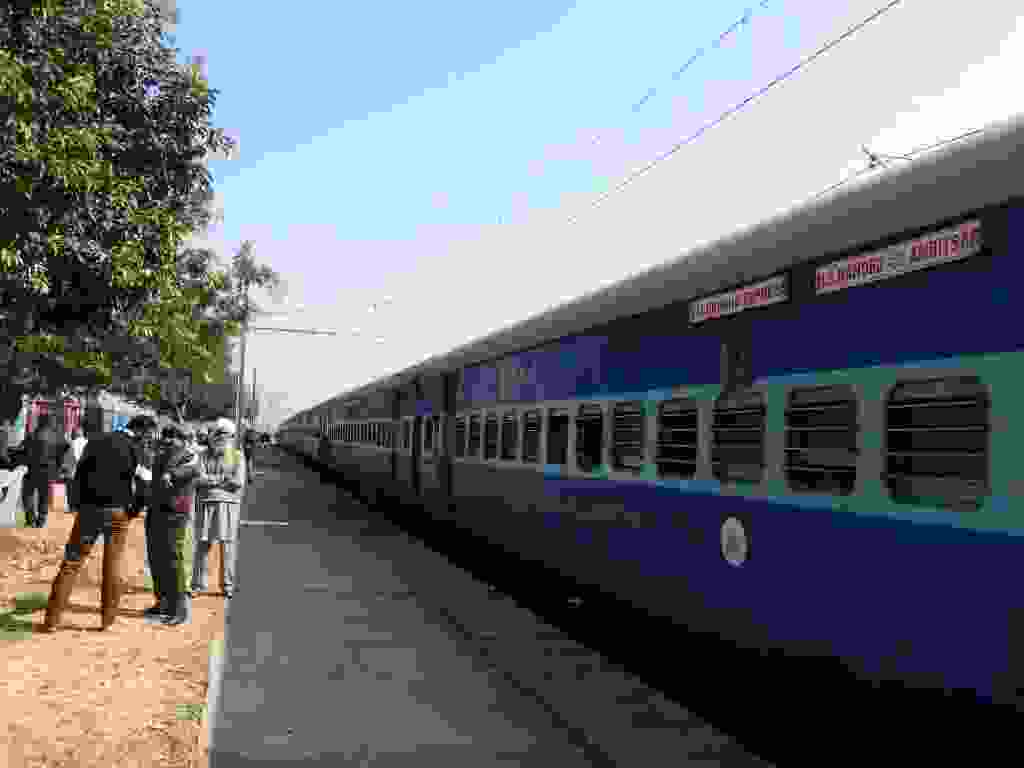
\includegraphics[width=\mywidth]{../wp-content/uploads/2015/12/wpid-oi000791-1024x768.jpg} \end{center}
\begin{center} 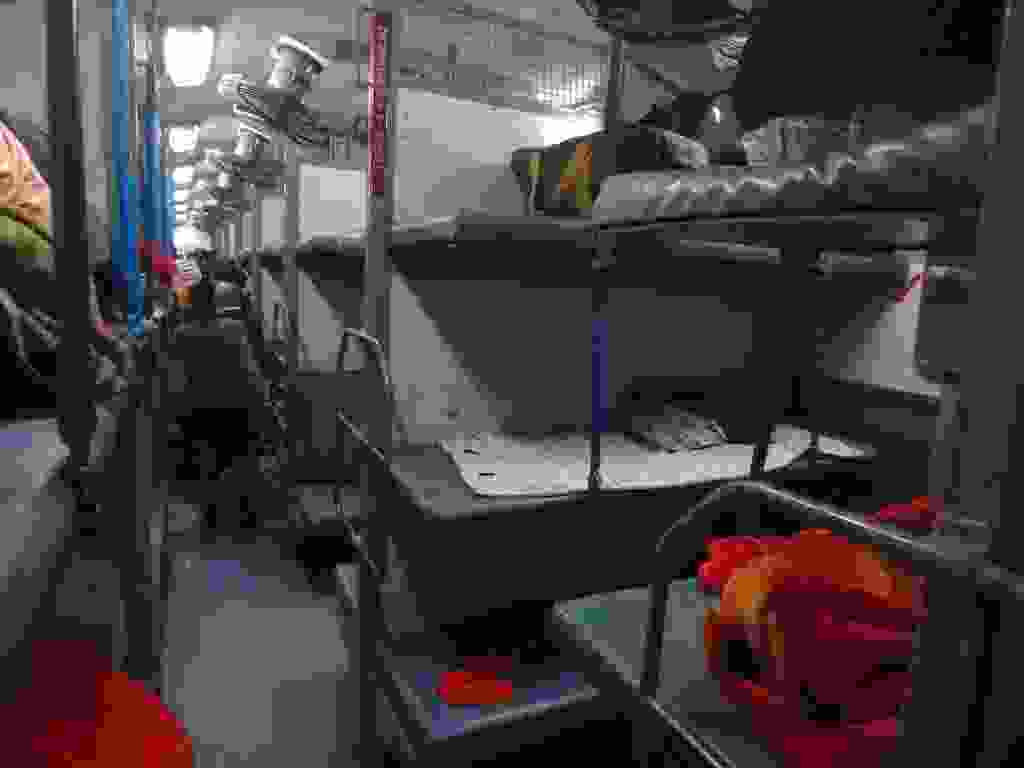
\includegraphics[width=\mywidth]{../wp-content/uploads/2015/12/wpid-oi000790-1024x768.jpg} \end{center}

Une nuit dans un dortoir à l'indienne : 1.4€
\begin{center} 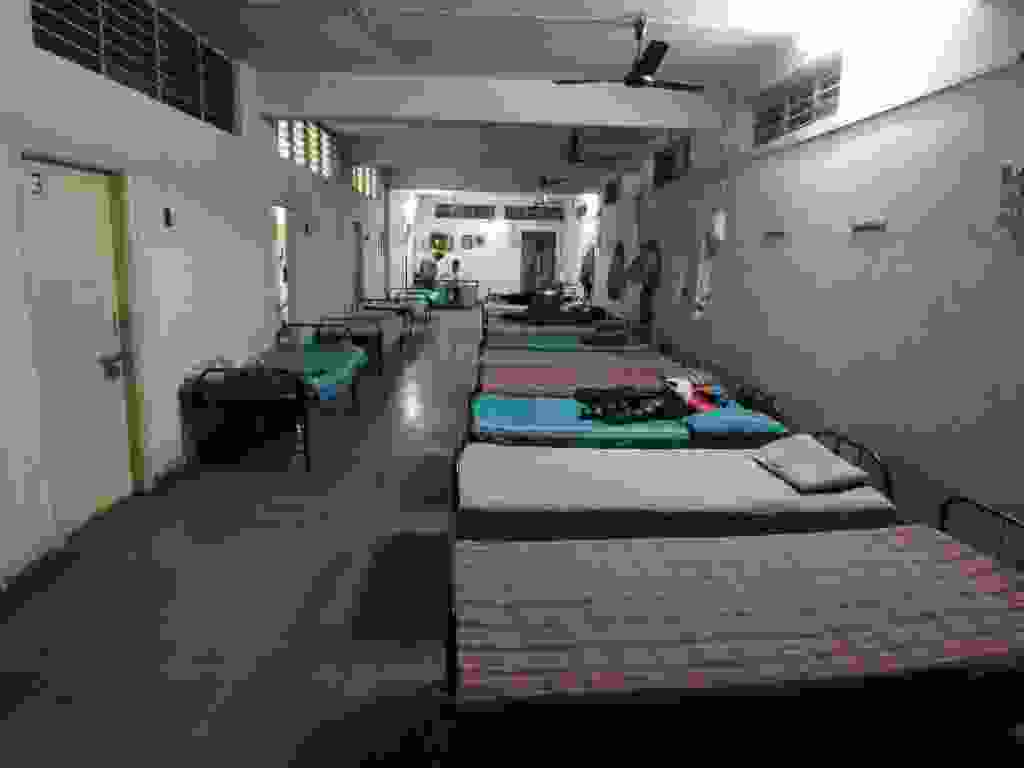
\includegraphics[width=\mywidth]{../wp-content/uploads/2015/12/wpid-oi000793-1024x768.jpg} \end{center}
\pagebreak

Ajanta à 90km d'Aurangabad : 30 grottes bouddhistes creusées dans la falaise entre le deuxième siècle avant J-C et le huitième siècle
\begin{center} 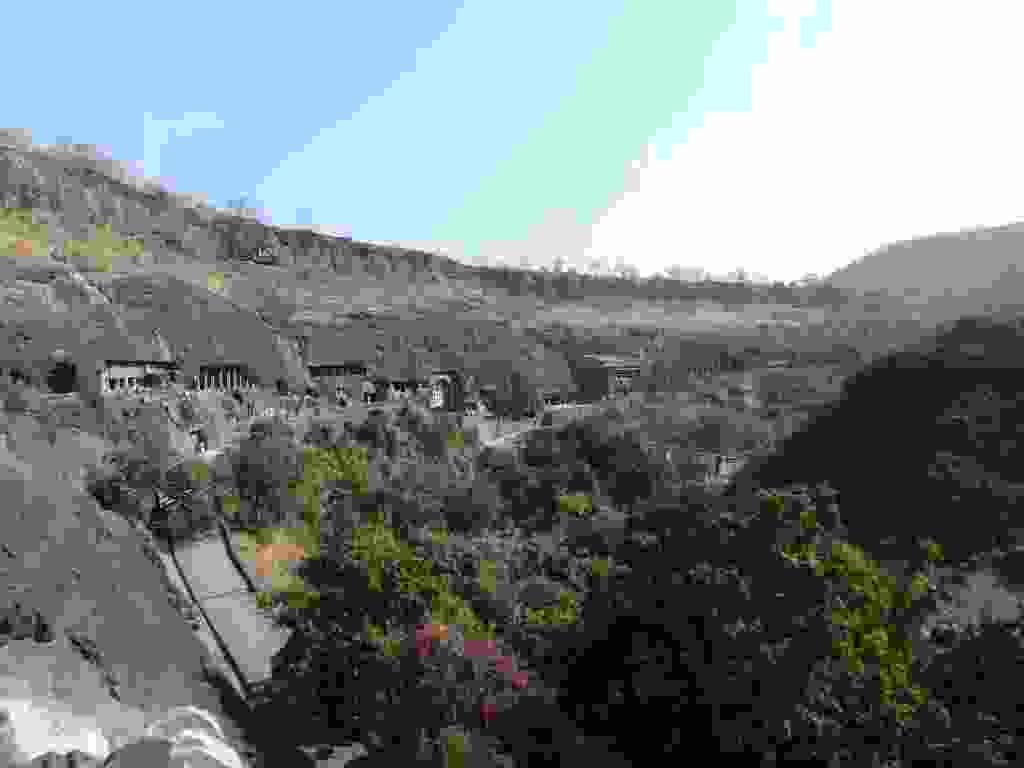
\includegraphics[width=\mywidth]{../wp-content/uploads/2015/12/PC151302-1024x768.jpg} \end{center}
\begin{center} 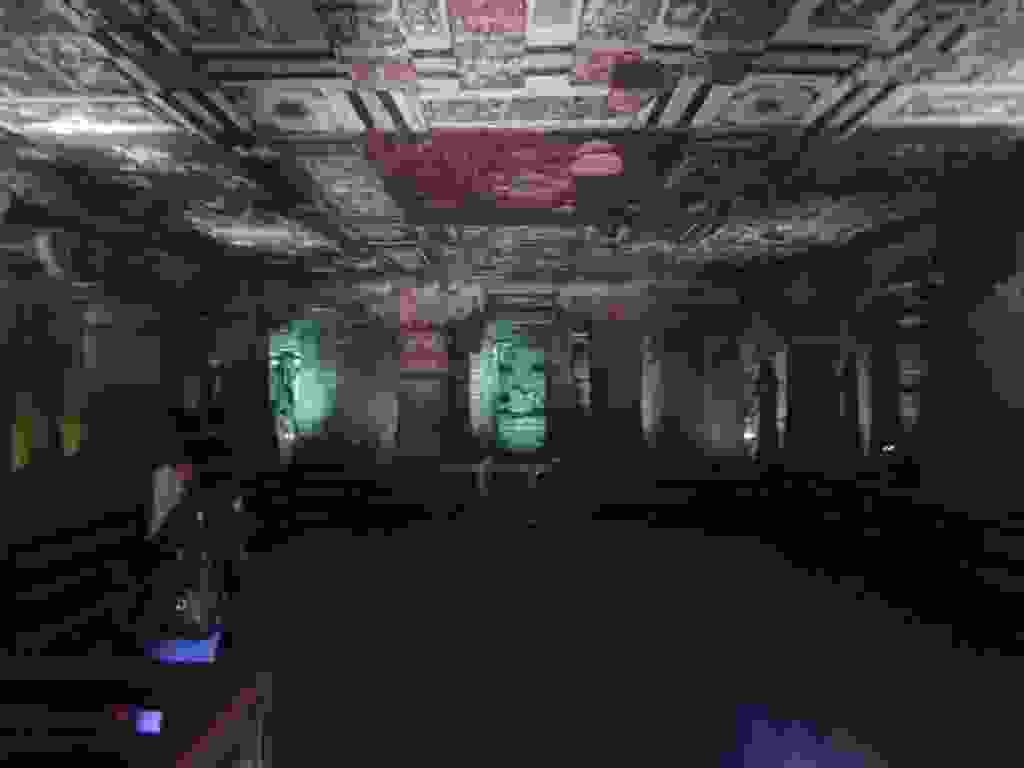
\includegraphics[width=\mywidth]{../wp-content/uploads/2015/12/PC151272-1024x768.jpg} \end{center}
\begin{center} 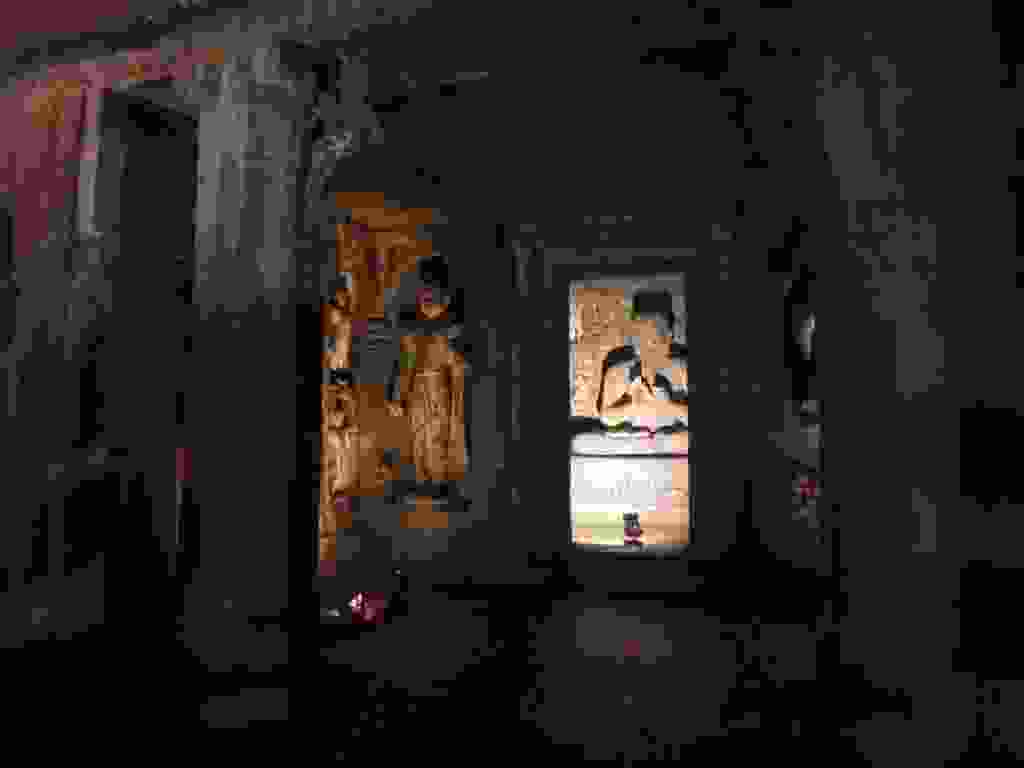
\includegraphics[width=\mywidth]{../wp-content/uploads/2015/12/PC151278-1024x768.jpg} \end{center}
\begin{center} 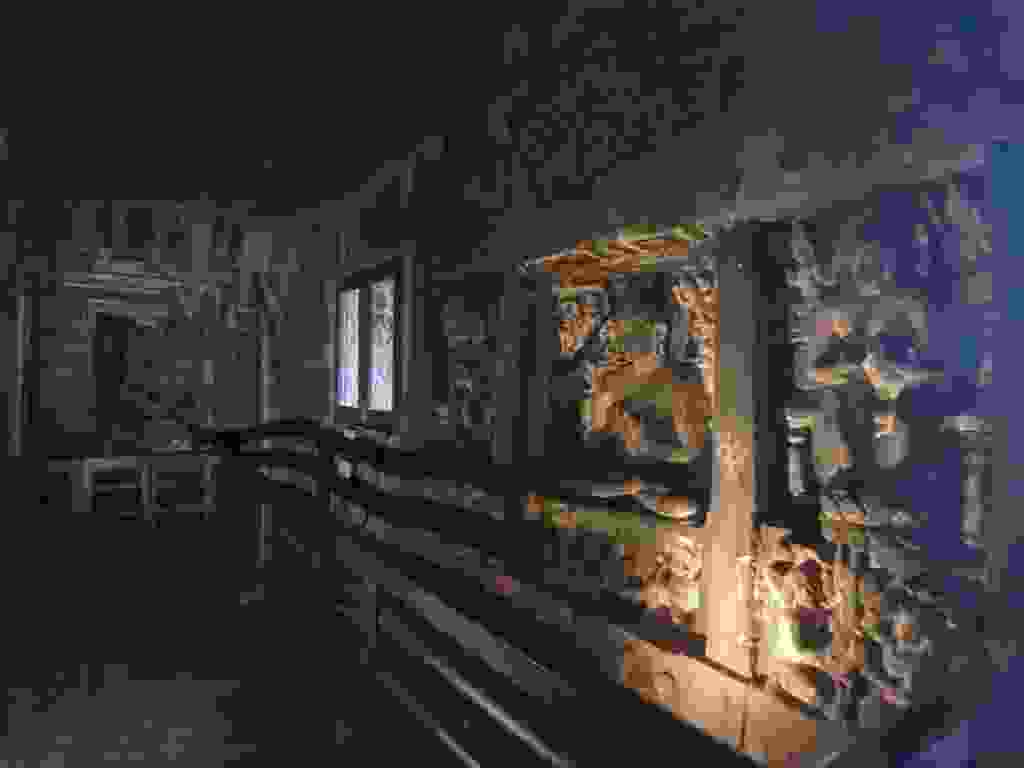
\includegraphics[width=\mywidth]{../wp-content/uploads/2015/12/PC151280-1024x768.jpg} \end{center}
\begin{center} 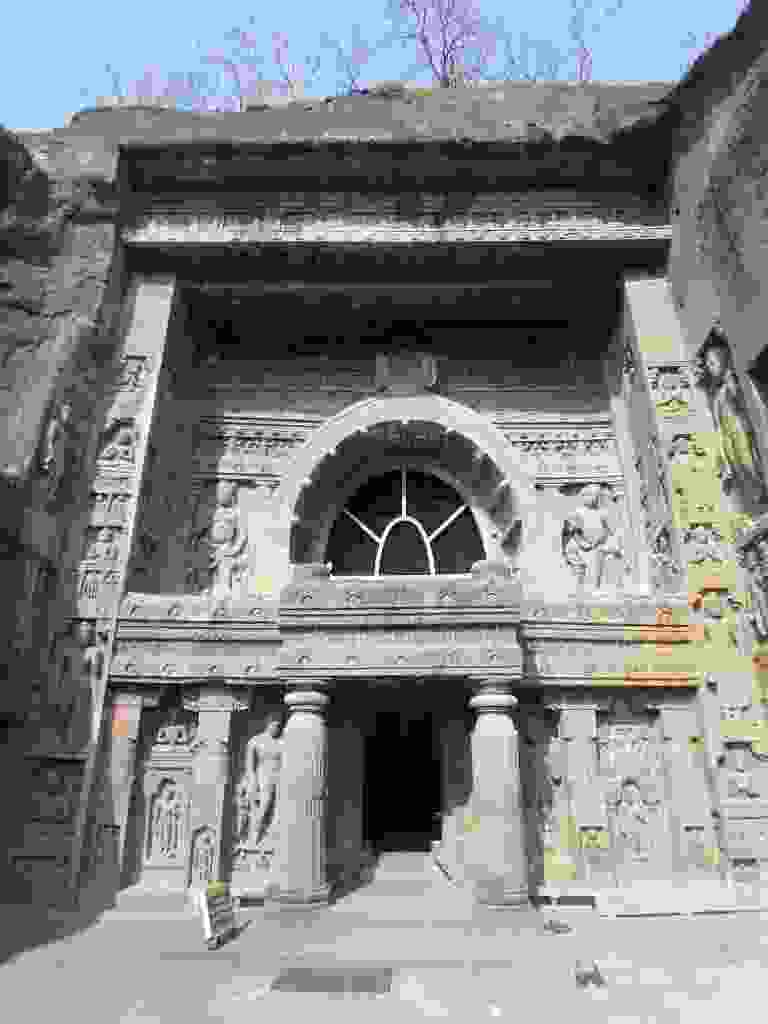
\includegraphics[width=0.6\textwidth]{../wp-content/uploads/2015/12/PC151297-768x1024.jpg} \end{center}
\begin{center} 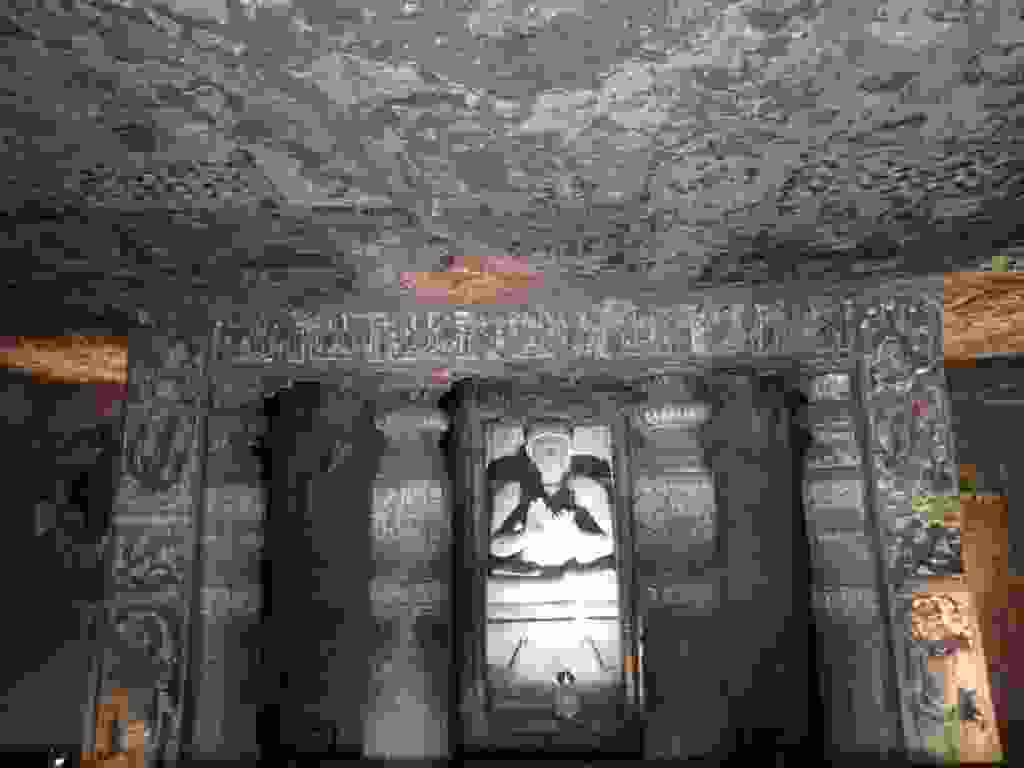
\includegraphics[width=\mywidth]{../wp-content/uploads/2015/12/PC151301-1024x768.jpg} \end{center}
\begin{center} 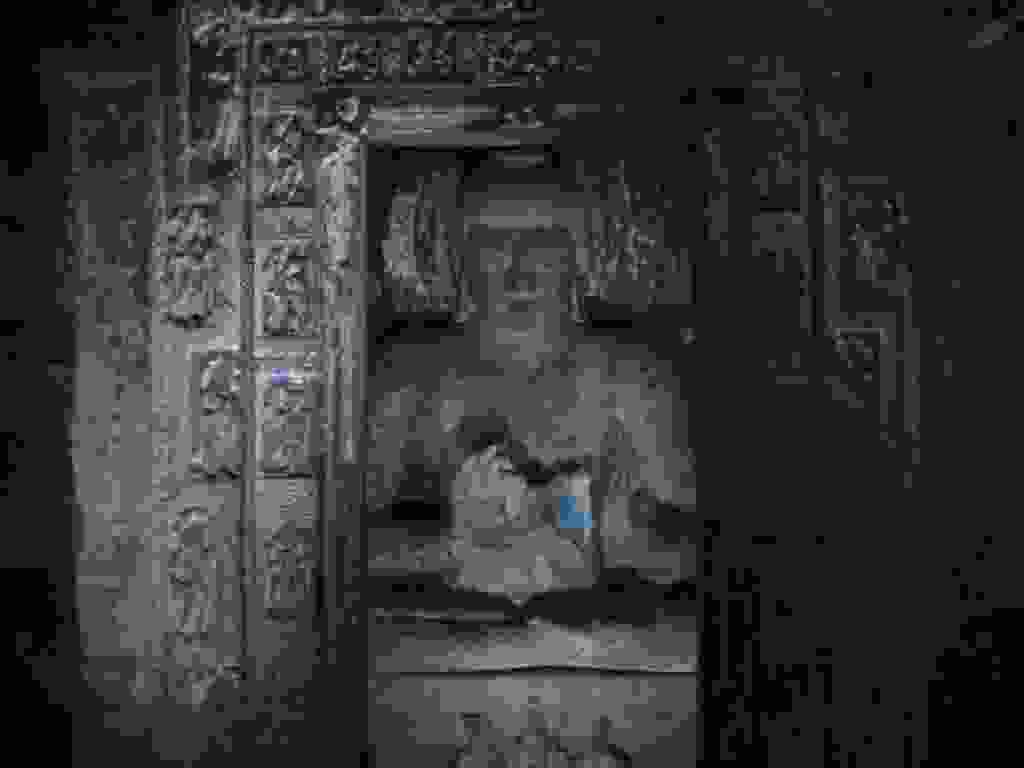
\includegraphics[width=\mywidth]{../wp-content/uploads/2015/12/PC151268-1024x768.jpg} \end{center}
\begin{center} 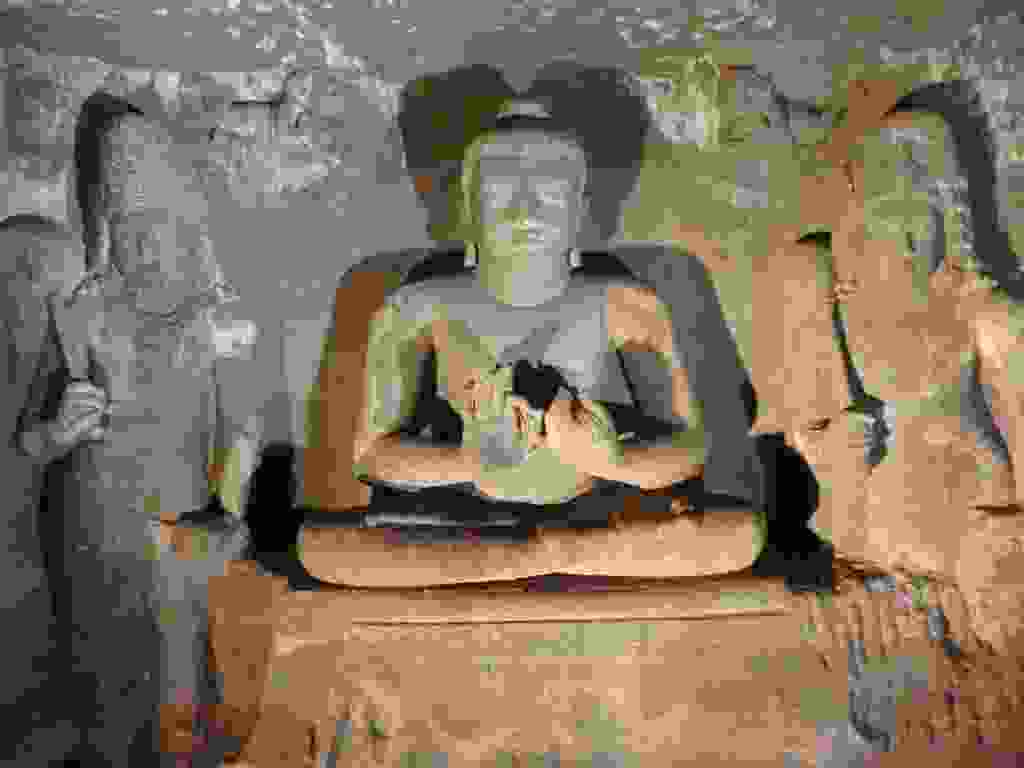
\includegraphics[width=\mywidth]{../wp-content/uploads/2015/12/PC151307-1024x768.jpg} \end{center}
\begin{center} 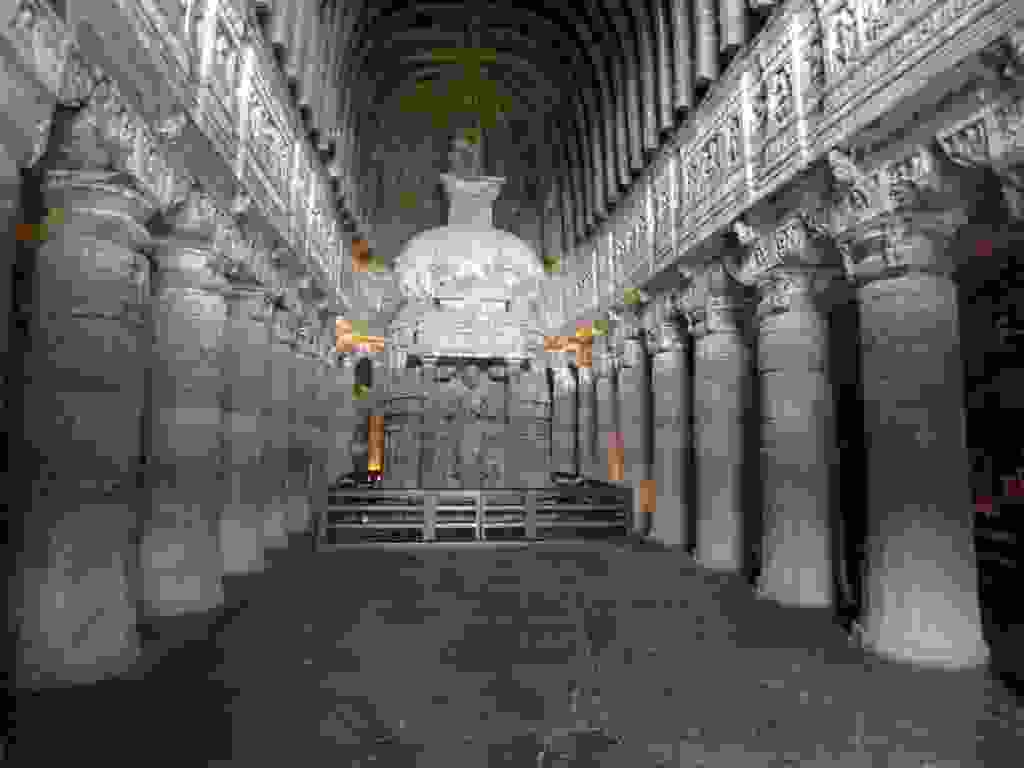
\includegraphics[width=\mywidth]{../wp-content/uploads/2015/12/PC151320-1024x768.jpg} \end{center}
\begin{center} 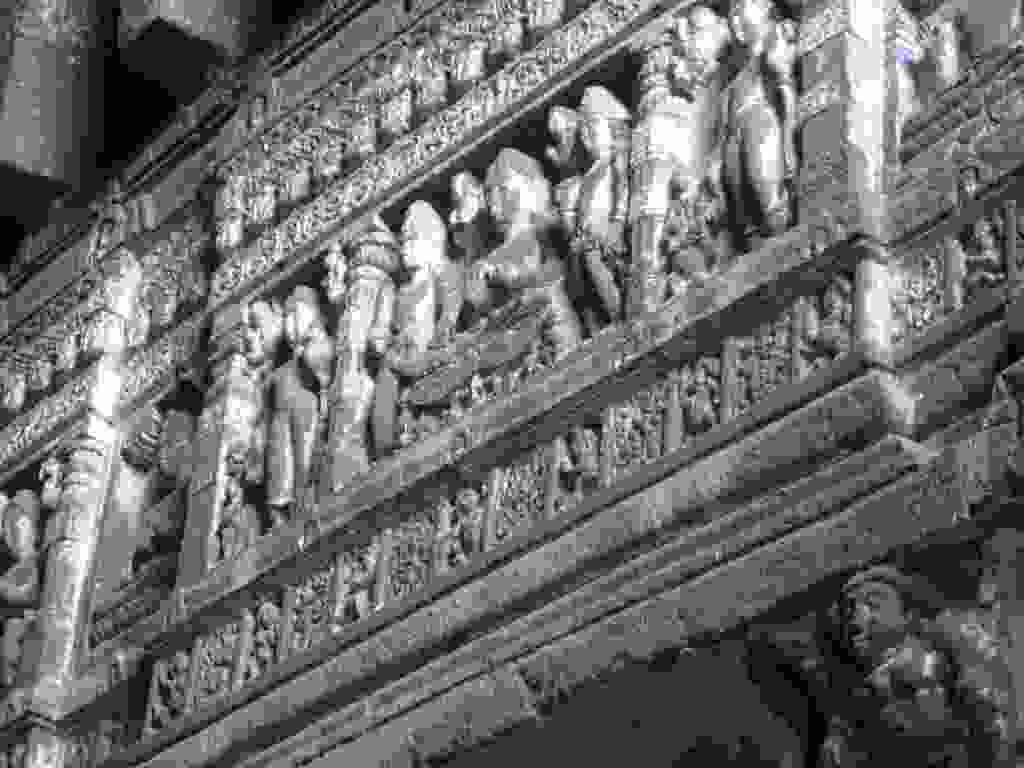
\includegraphics[width=\mywidth]{../wp-content/uploads/2015/12/PC151321-1024x768.jpg} \end{center}
\pagebreak

Restes de peintures
\begin{center} 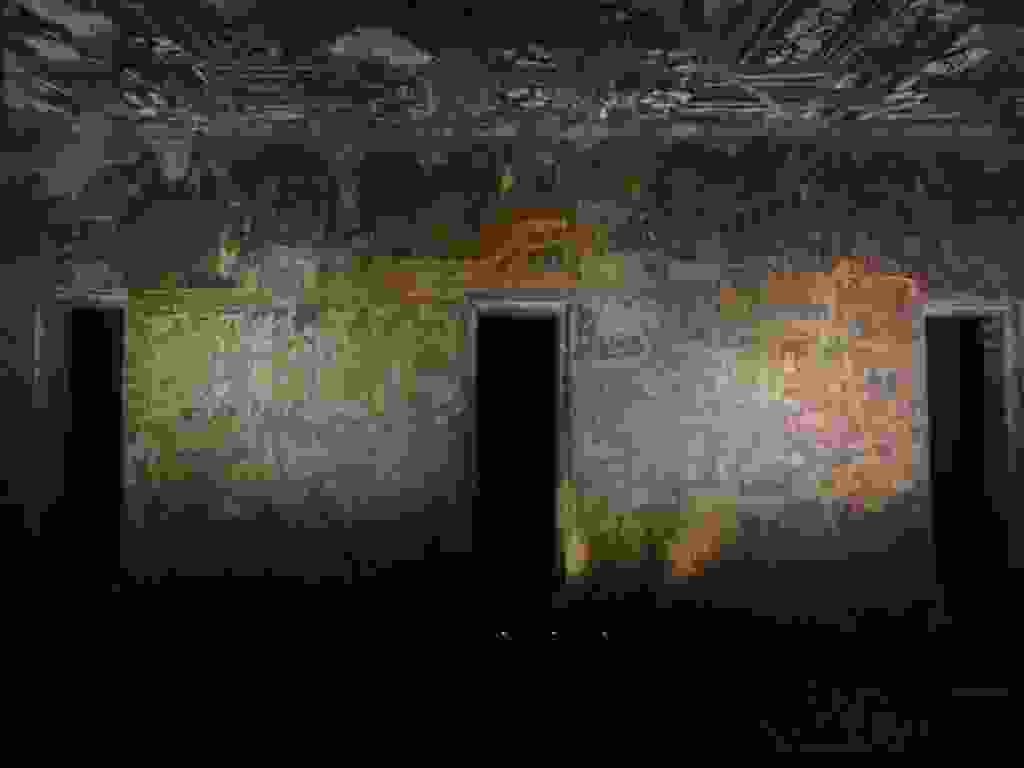
\includegraphics[width=\mywidth]{../wp-content/uploads/2015/12/PC151269-1024x768.jpg} \end{center}

Beau site naturel autour des grottes, il doit y avoir de belles cascades pendant la saison des pluies 
\begin{center} 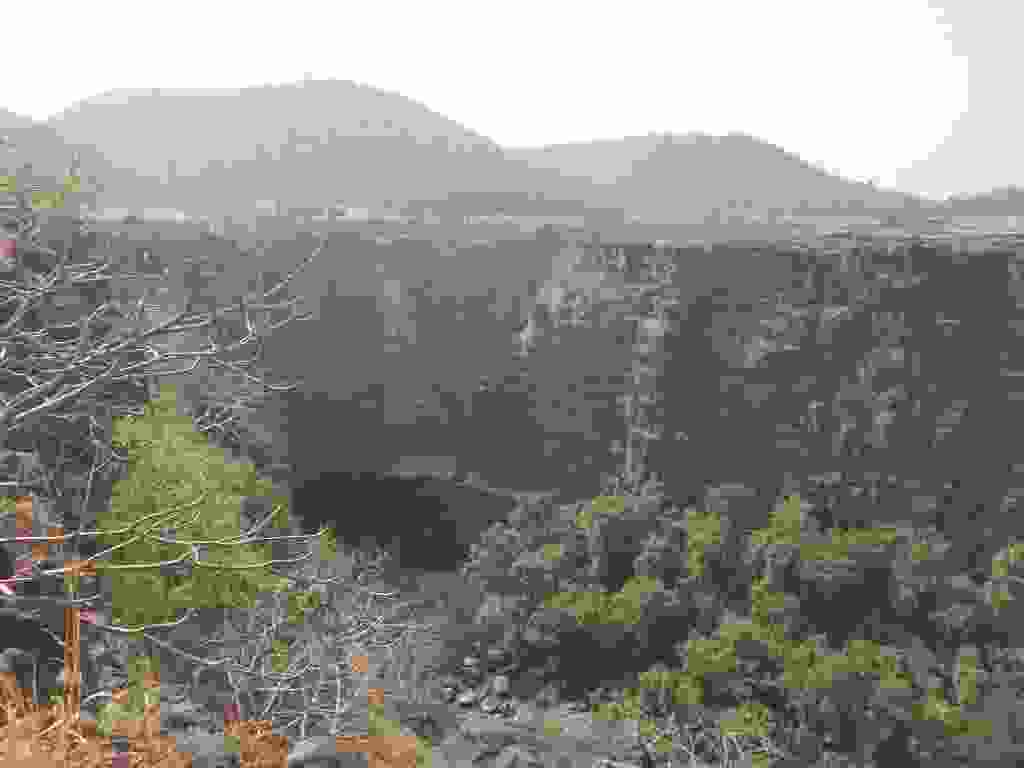
\includegraphics[width=\mywidth]{../wp-content/uploads/2015/12/PC151325-1024x768.jpg} \end{center}
\pagebreak

Je rencontre un indien qui me fait visiter son village juste au dessus d'Ajanta : très tranquille, pas de voiture donc pas de klaxons incessants comme partout ailleurs 
\begin{center} 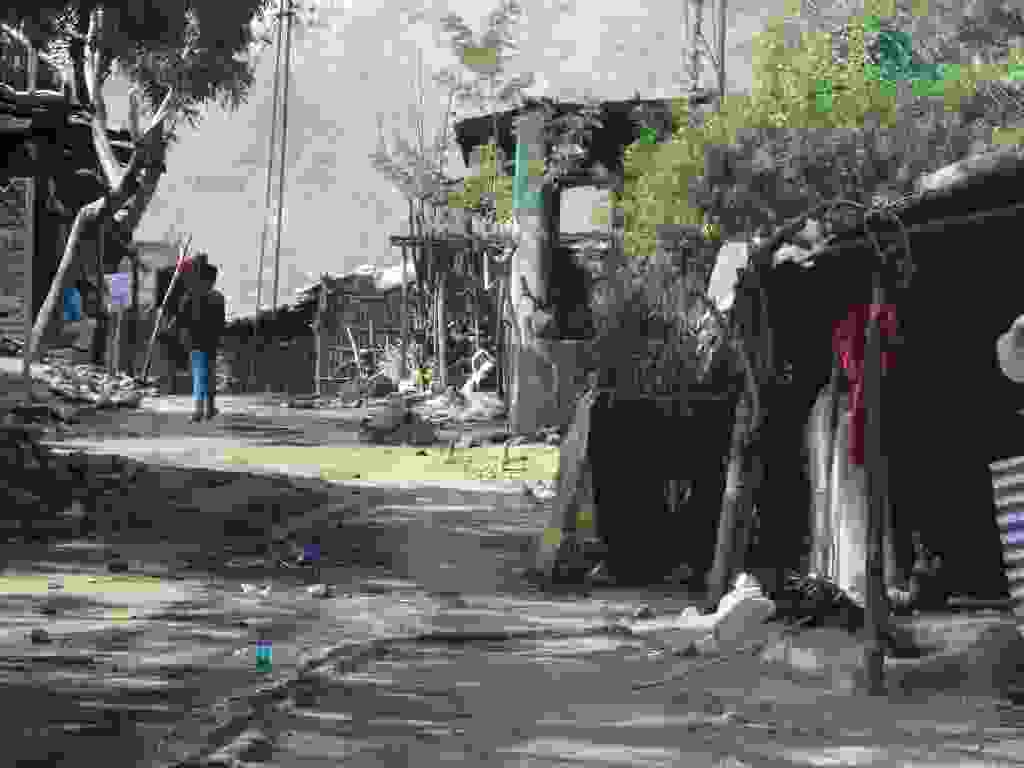
\includegraphics[width=\mywidth]{../wp-content/uploads/2015/12/PC151327-1024x768.jpg} \end{center}
\begin{center} 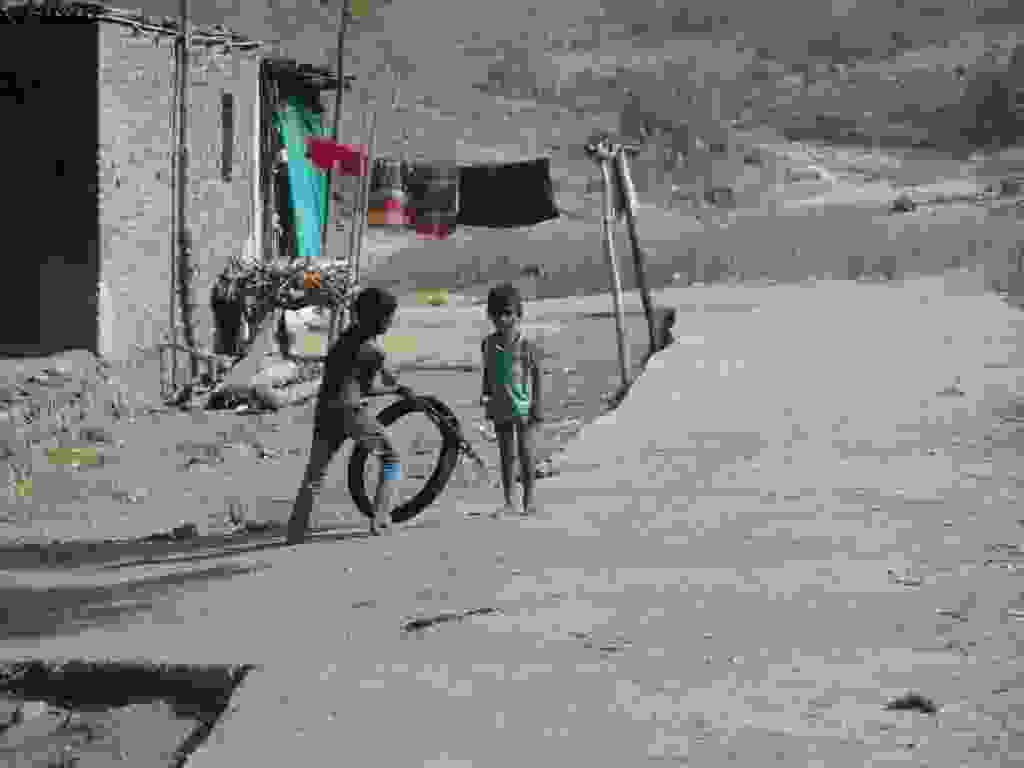
\includegraphics[width=\mywidth]{../wp-content/uploads/2015/12/PC151328-1024x768.jpg} \end{center}
\begin{center} 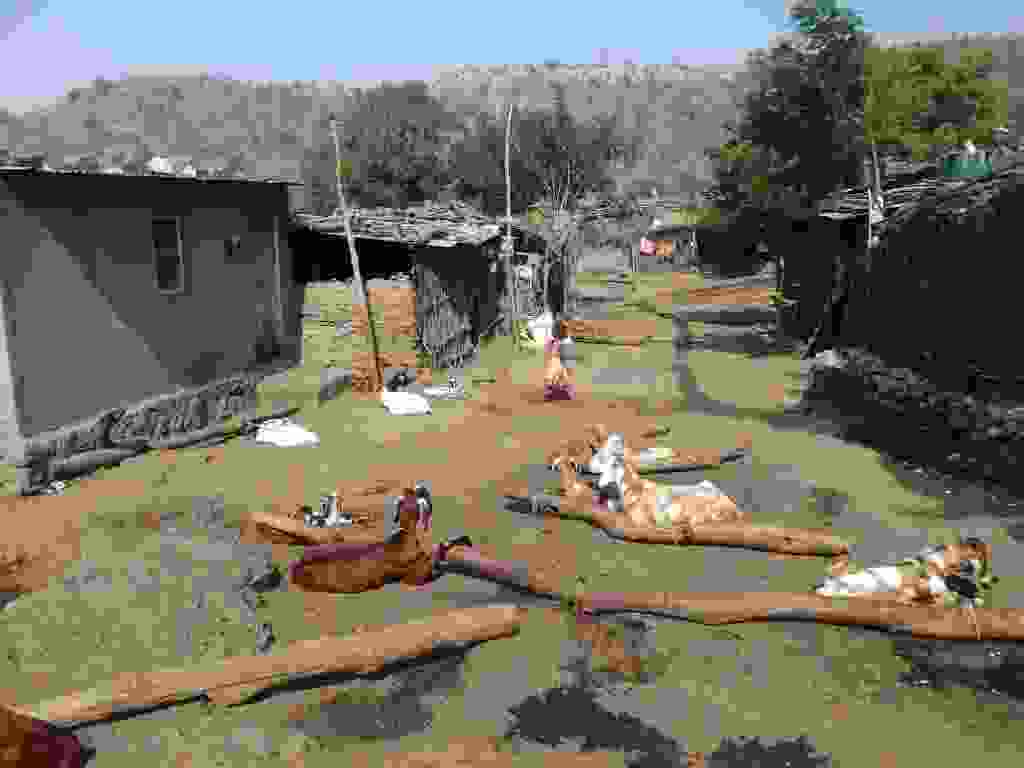
\includegraphics[width=\mywidth]{../wp-content/uploads/2015/12/PC151329-1024x768.jpg} \end{center}

L'école du village 
\begin{center} 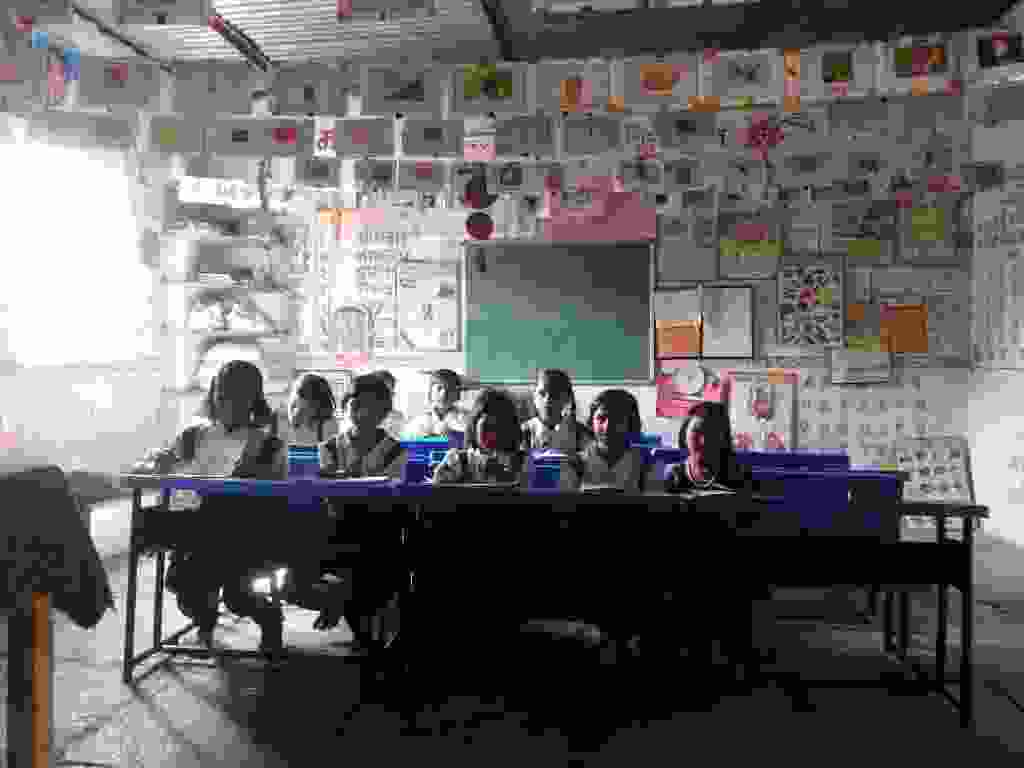
\includegraphics[width=\mywidth]{../wp-content/uploads/2015/12/PC151330-1024x768.jpg} \end{center}
\pagebreak

Ellora juste à côté d'Aurangabad : un mélange de grottes hindoues, jainistes et bouddhistes 

Temple hindou de Kailasanatha, entièrement excavé dans la falaise 
\begin{center} 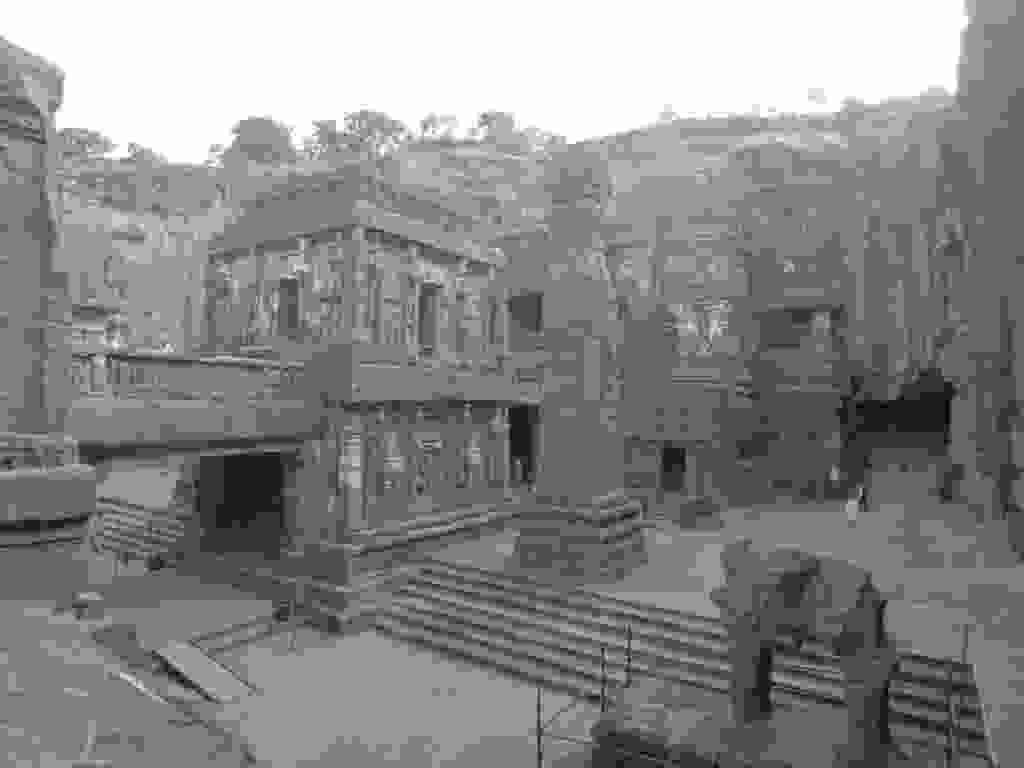
\includegraphics[width=\mywidth]{../wp-content/uploads/2015/12/PC161360-1024x768.jpg} \end{center}
\begin{center} 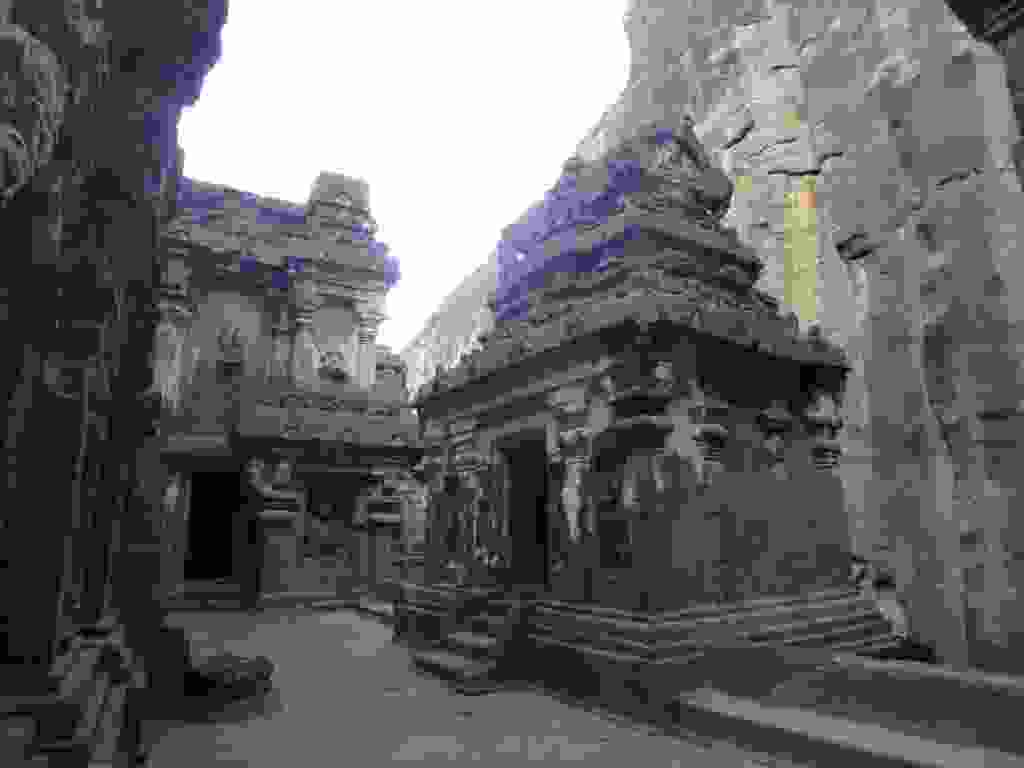
\includegraphics[width=\mywidth]{../wp-content/uploads/2015/12/PC161356-1024x768.jpg} \end{center}
\pagebreak

Groupe de 4 grottes jainistes 
\begin{center} 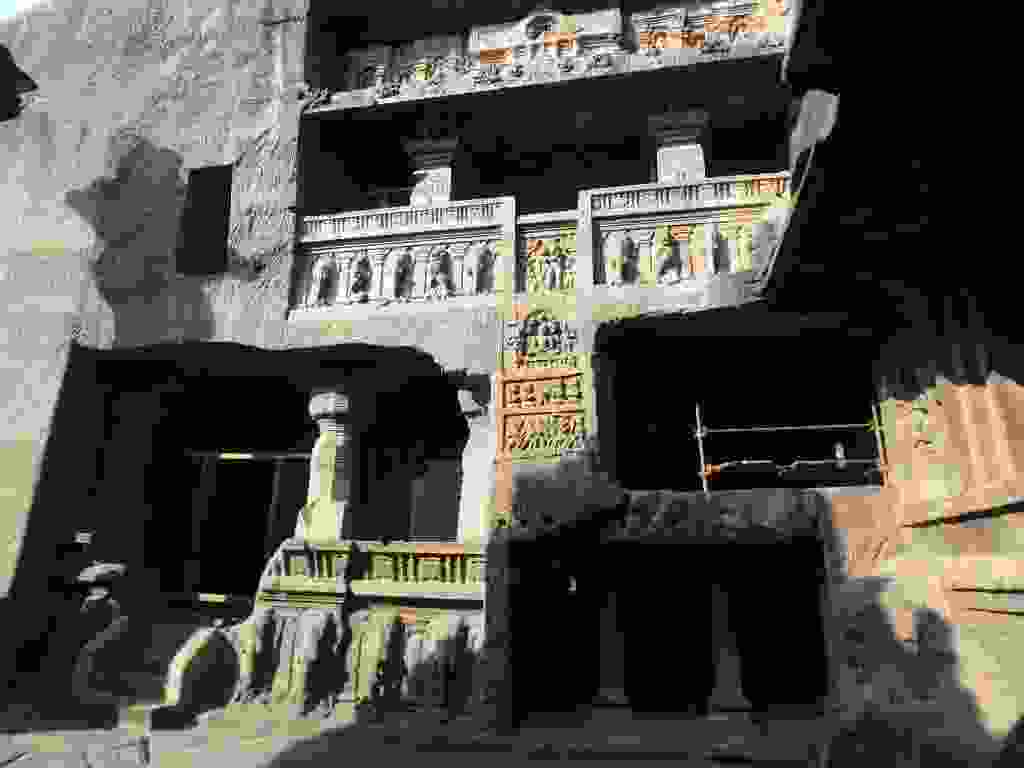
\includegraphics[width=\mywidth]{../wp-content/uploads/2015/12/PC161387-1024x768.jpg} \end{center}
\begin{center} 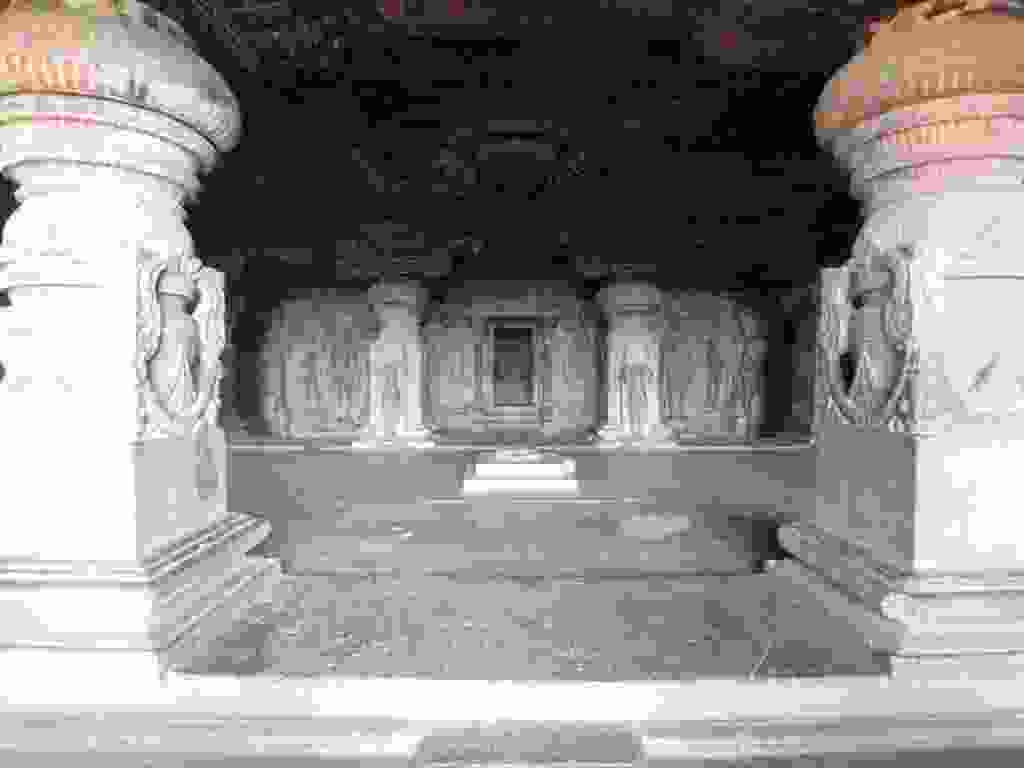
\includegraphics[width=\mywidth]{../wp-content/uploads/2015/12/PC161390-1024x768.jpg} \end{center}
\begin{center} 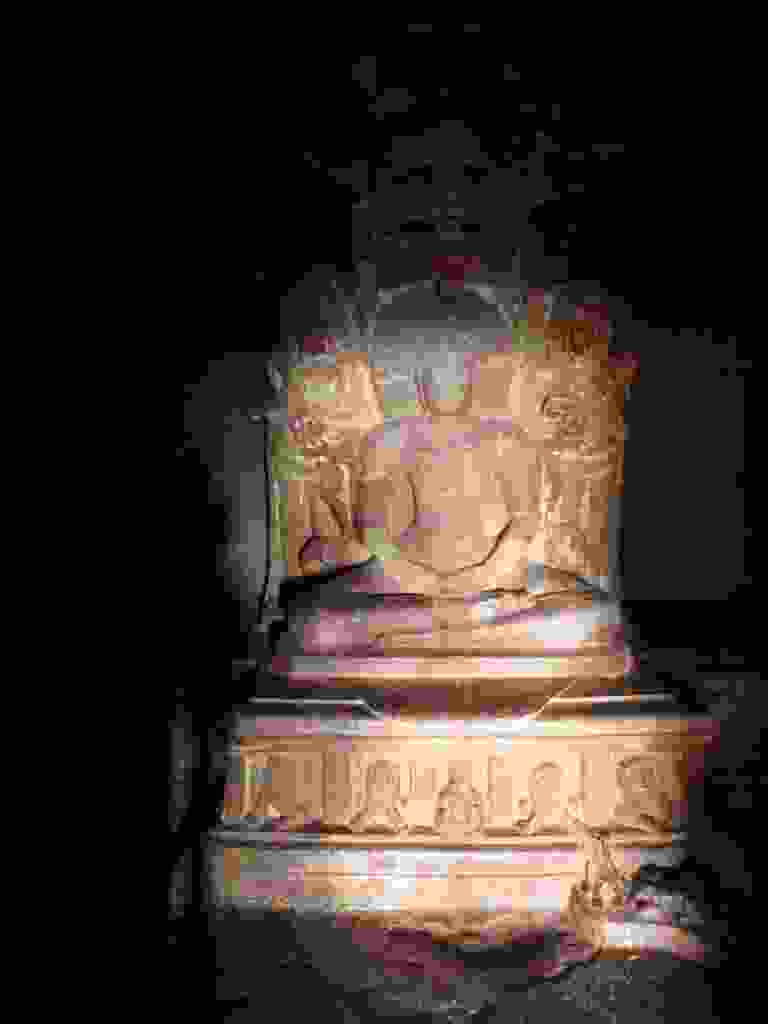
\includegraphics[width=0.6\textwidth]{../wp-content/uploads/2015/12/PC161392-768x1024.jpg} \end{center}

Une dizaines de grottes bouddhistes, ayant servies de temple ou de monastère, ça attire des touristes particuliers 
\begin{center} 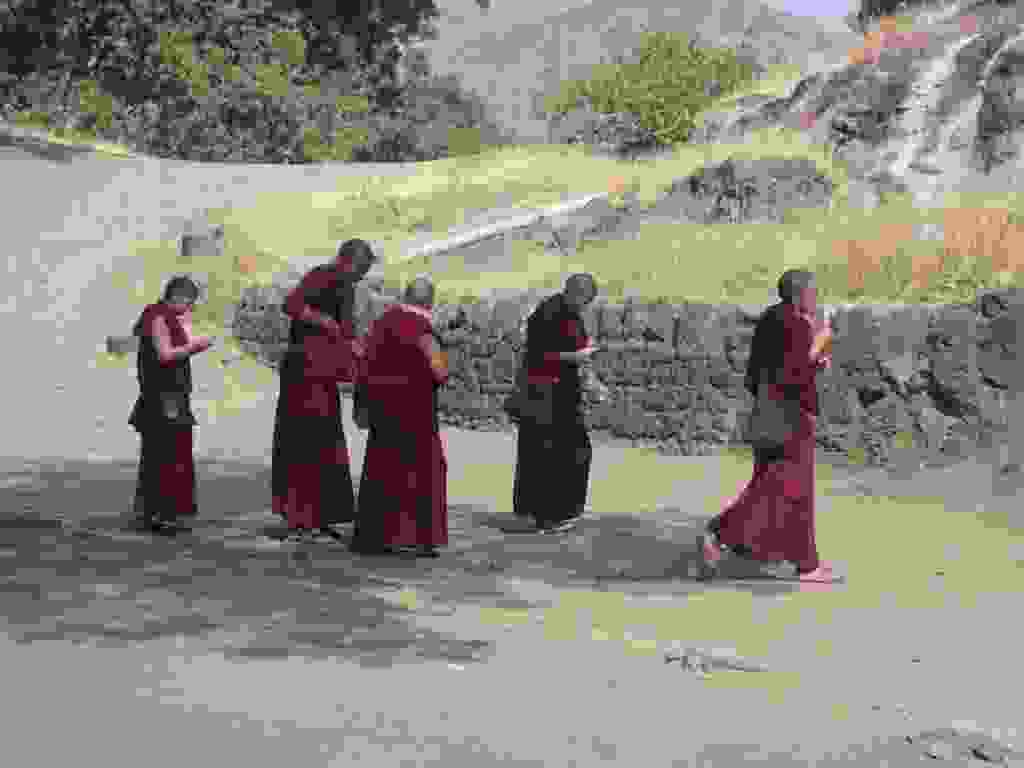
\includegraphics[width=\mywidth]{../wp-content/uploads/2015/12/PC161409-1024x768.jpg} \end{center}
\begin{center} 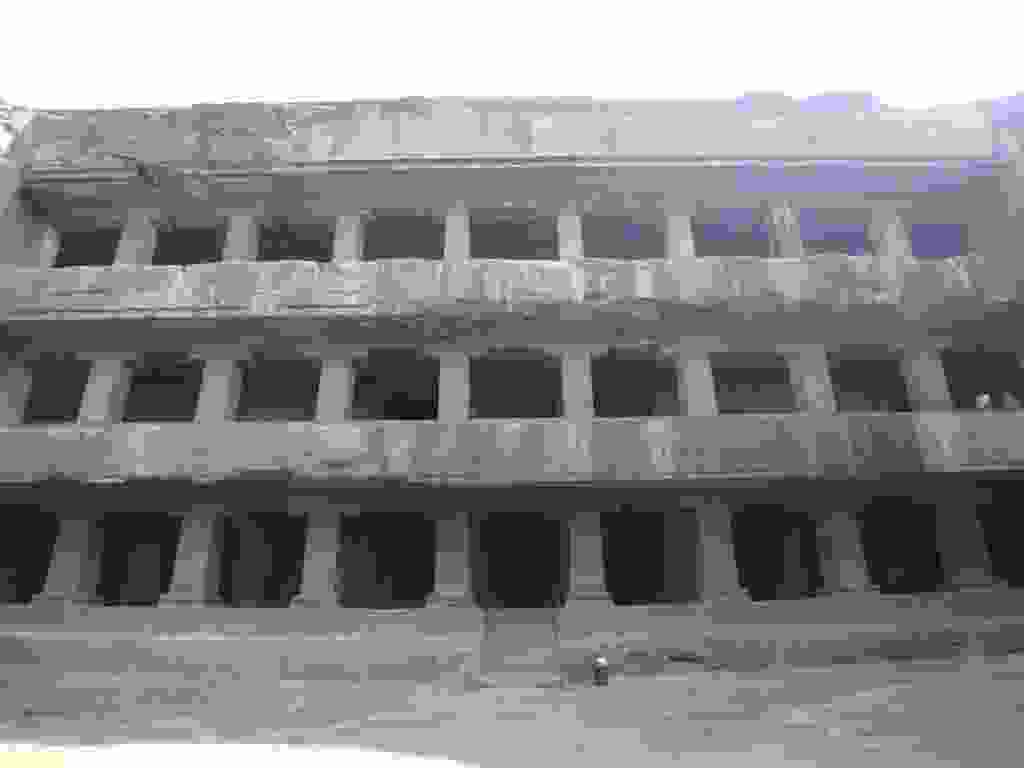
\includegraphics[width=\mywidth]{../wp-content/uploads/2015/12/PC161410-1024x768.jpg} \end{center}
\begin{center} 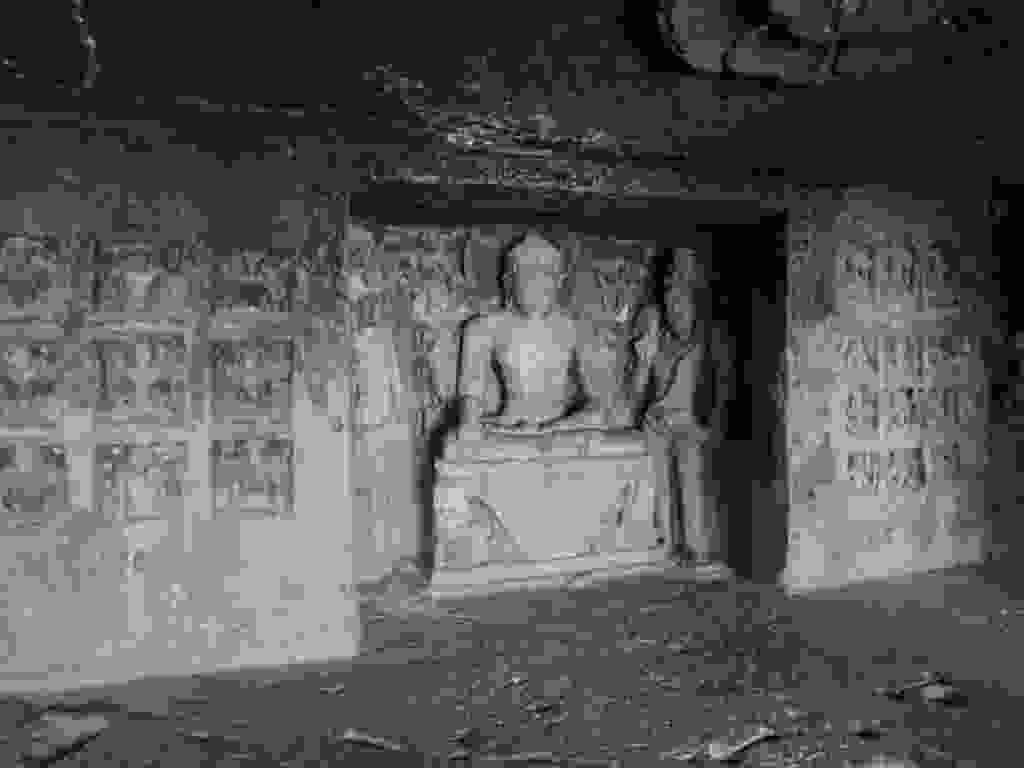
\includegraphics[width=\mywidth]{../wp-content/uploads/2015/12/PC161411-1024x768.jpg} \end{center}
\begin{center} 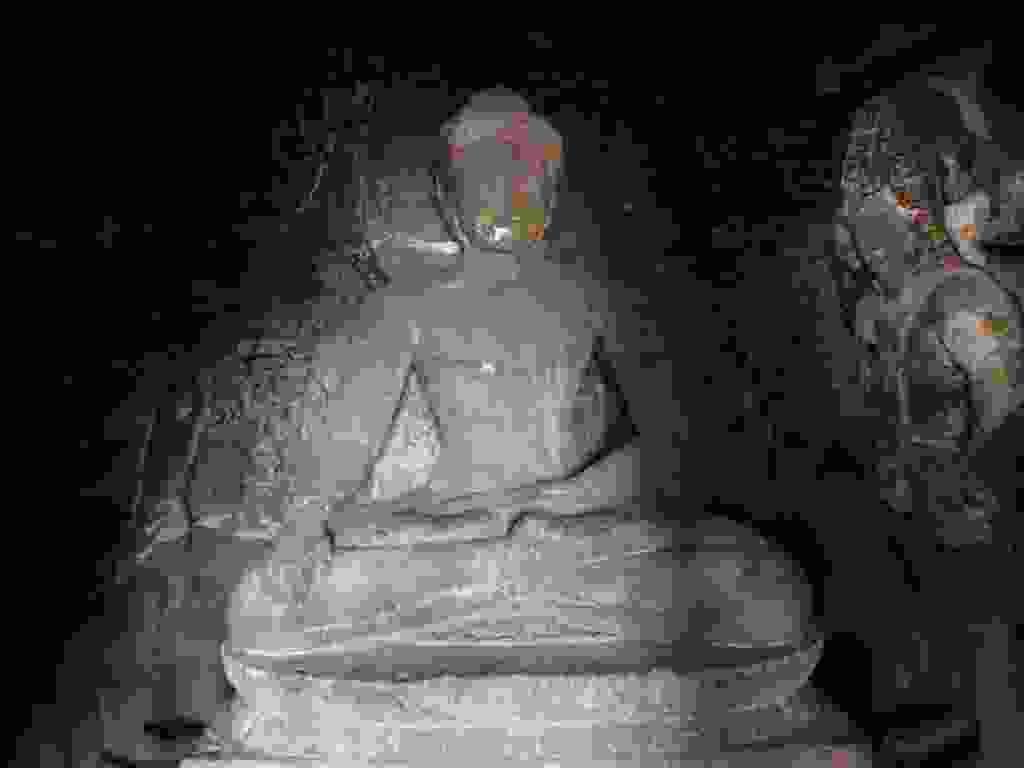
\includegraphics[width=\mywidth]{../wp-content/uploads/2015/12/PC161416-1024x768.jpg} \end{center}
\begin{center} 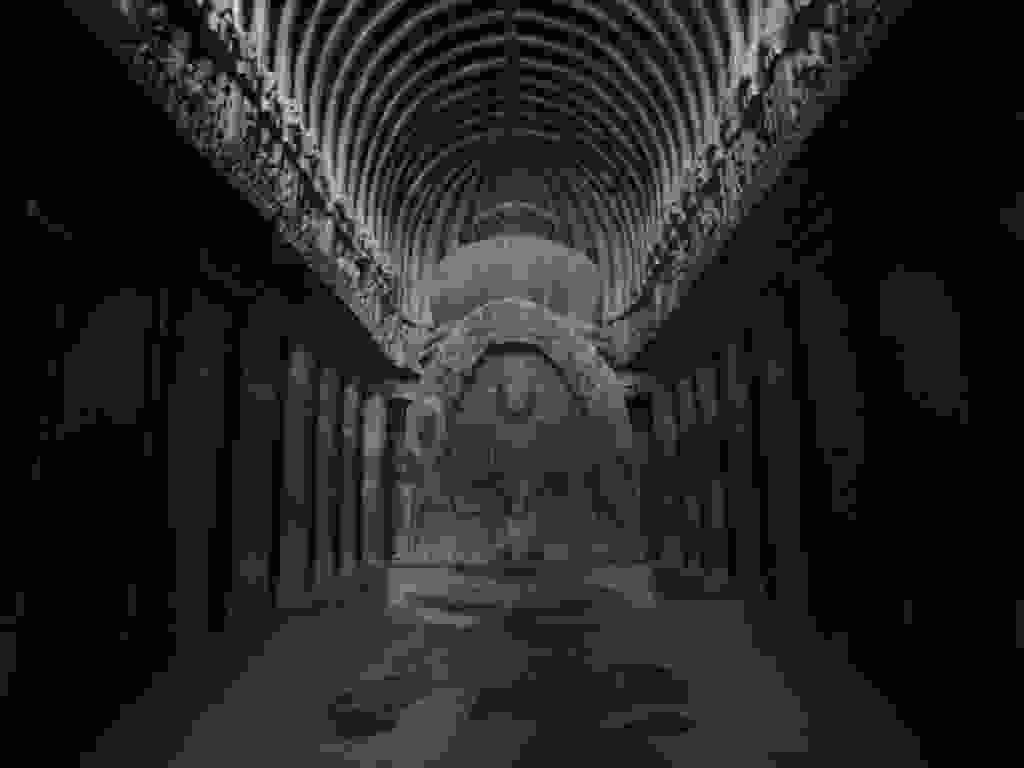
\includegraphics[width=\mywidth]{../wp-content/uploads/2015/12/PC161418-1024x768.jpg} \end{center}
\begin{center} 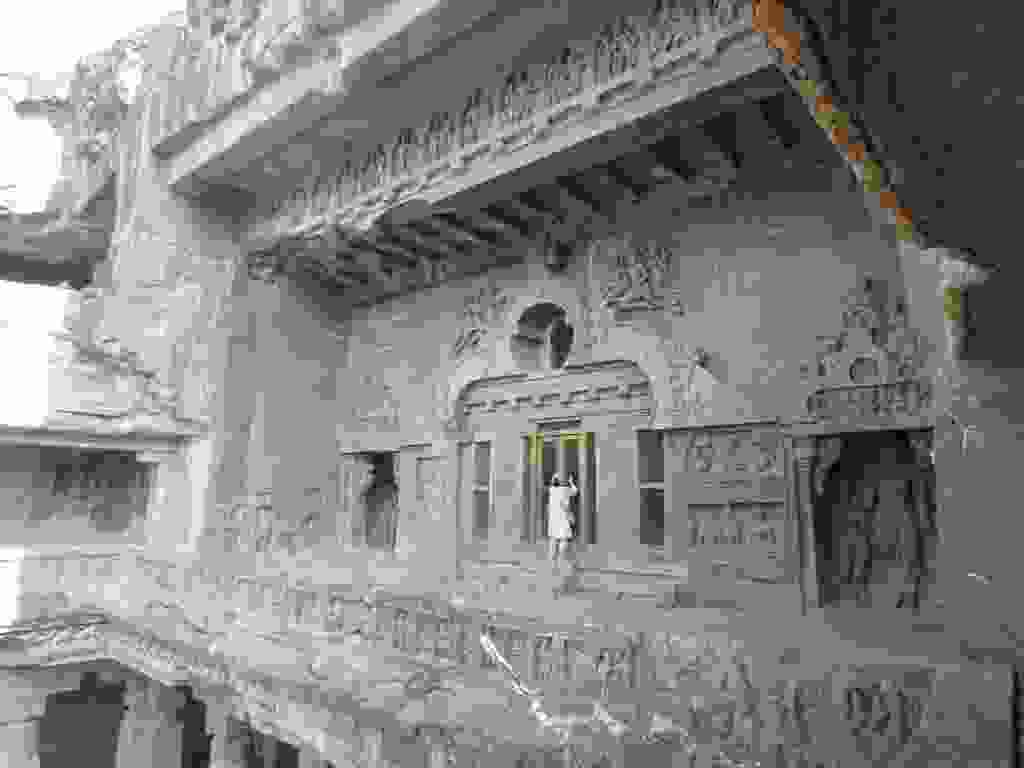
\includegraphics[width=\mywidth]{../wp-content/uploads/2015/12/PC161420-1024x768.jpg} \end{center}
\begin{center} 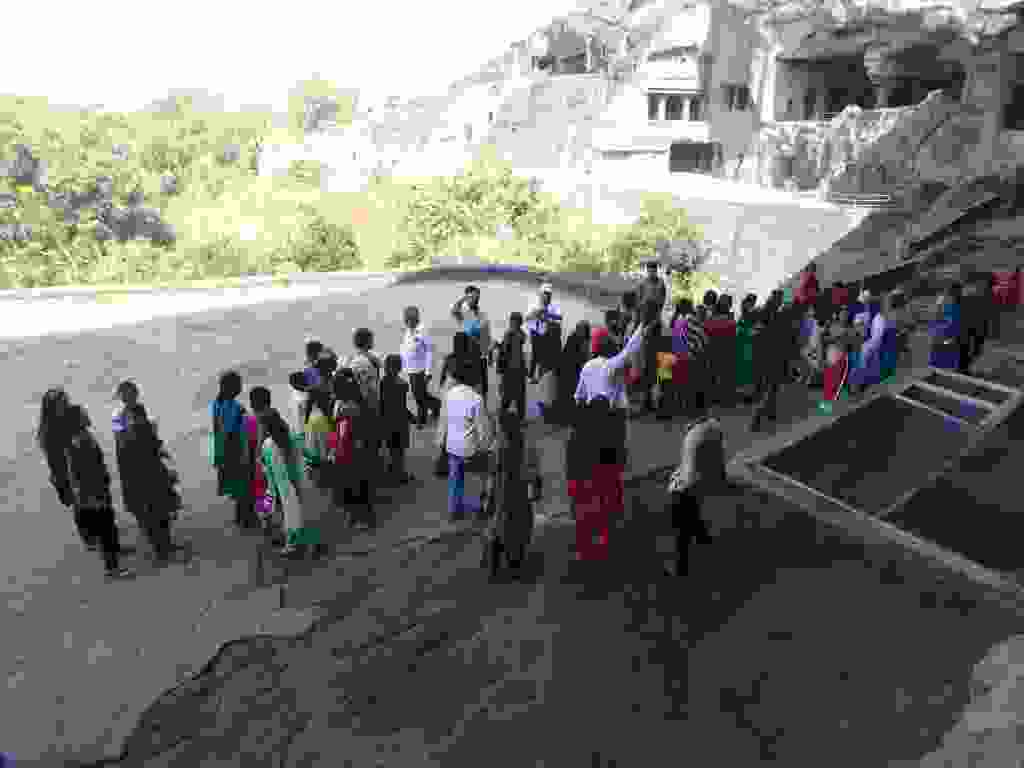
\includegraphics[width=\mywidth]{../wp-content/uploads/2015/12/PC161428-1024x768.jpg} \end{center}
\pagebreak


Je prends ensuite le bus pour rejoindre le village d'Hampi, il m'avait été conseillé par plusieurs voyageurs que j'ai rencontrés 
\begin{center} 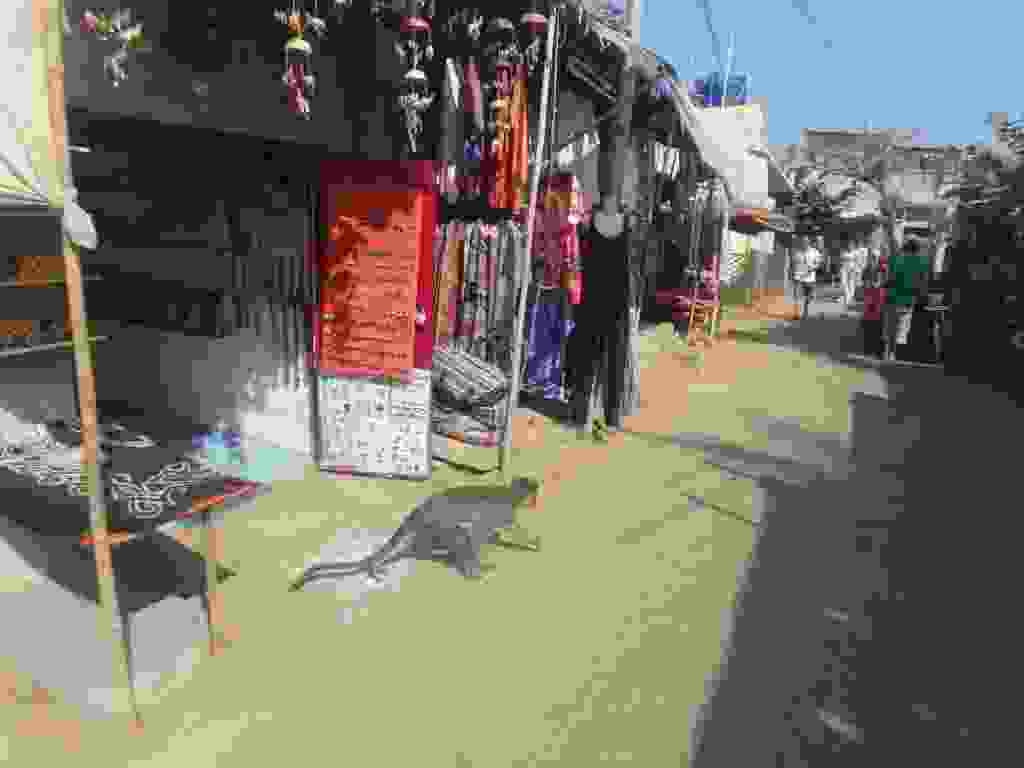
\includegraphics[width=\mywidth]{../wp-content/uploads/2015/12/PC181547-1024x768.jpg} \end{center}

Cadre naturel très particulier : des cailloux partout 
\begin{center} 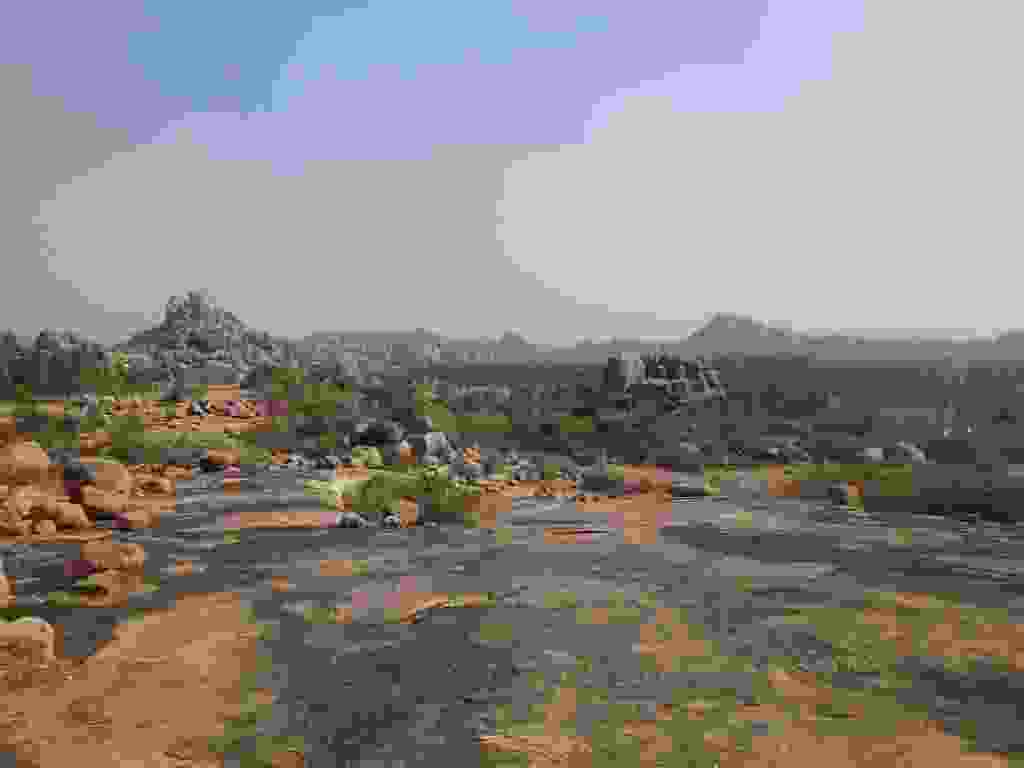
\includegraphics[width=\mywidth]{../wp-content/uploads/2015/12/PC171439-1024x768.jpg} \end{center}
\begin{center} 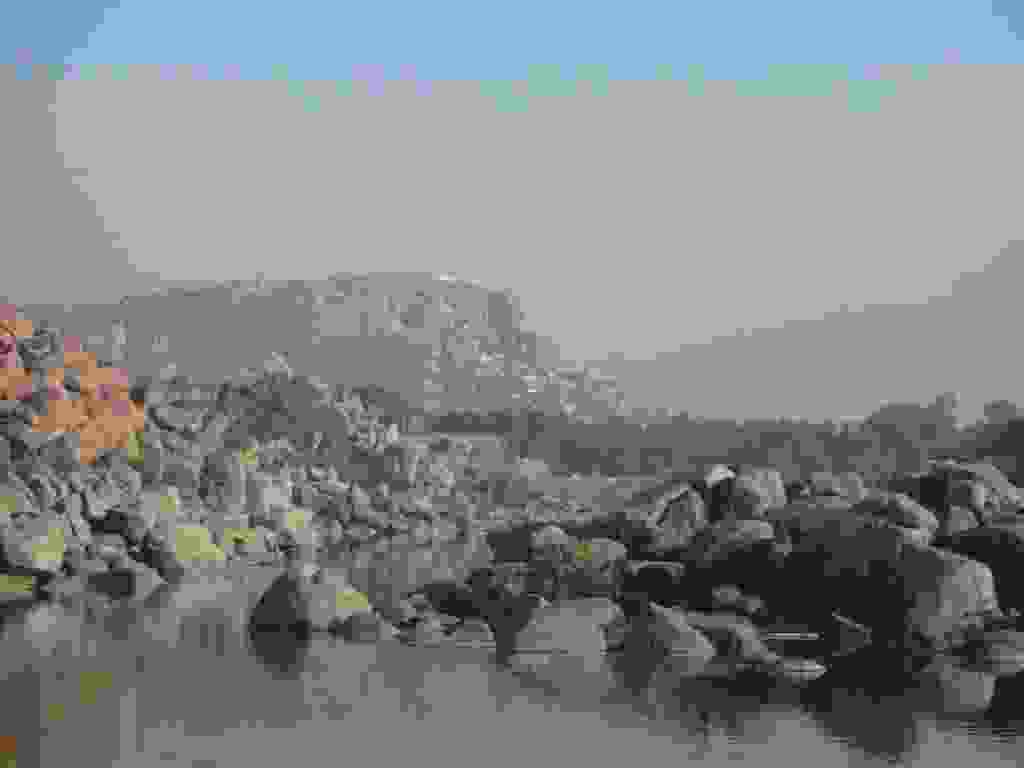
\includegraphics[width=\mywidth]{../wp-content/uploads/2015/12/PC181469-1024x768.jpg} \end{center}
\begin{center} 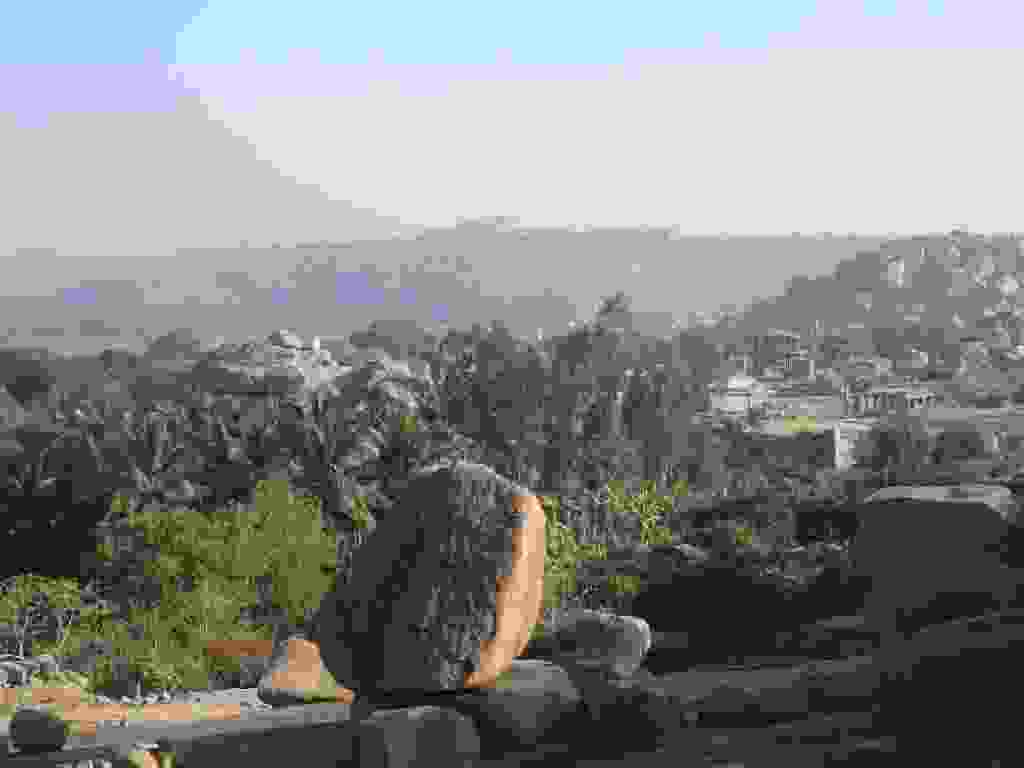
\includegraphics[width=\mywidth]{../wp-content/uploads/2015/12/PC181478-1024x768.jpg} \end{center}
\begin{center} 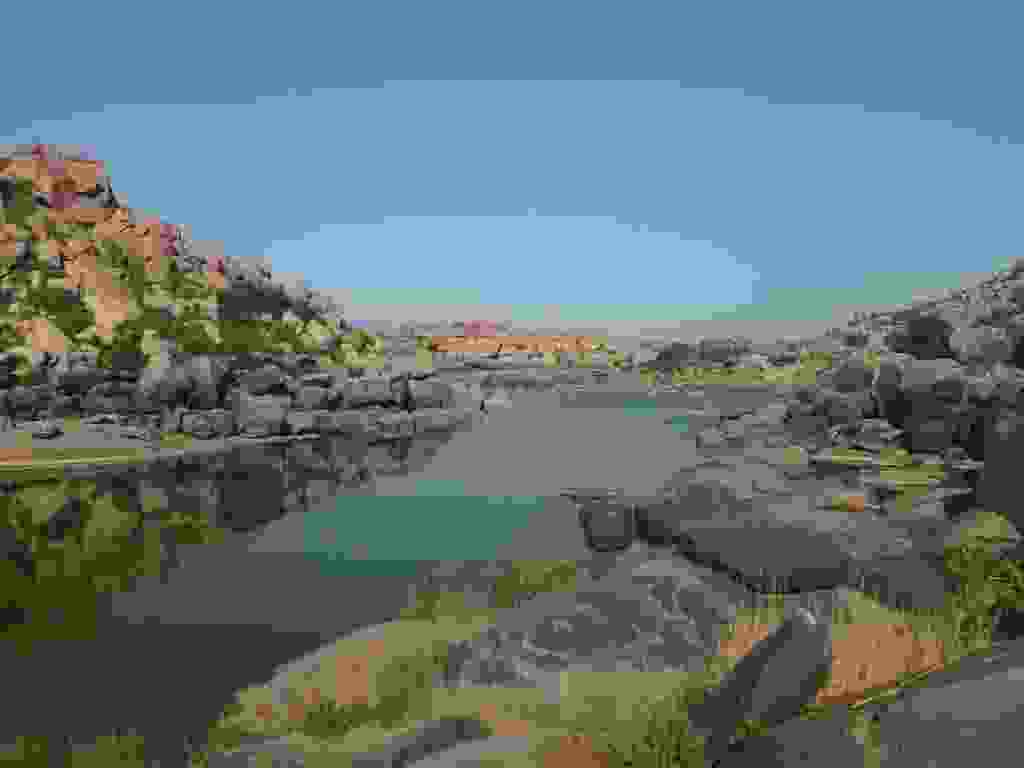
\includegraphics[width=\mywidth]{../wp-content/uploads/2015/12/PC181550-1024x768.jpg} \end{center}

Monkey temple en haut d'une colline 
\begin{center} 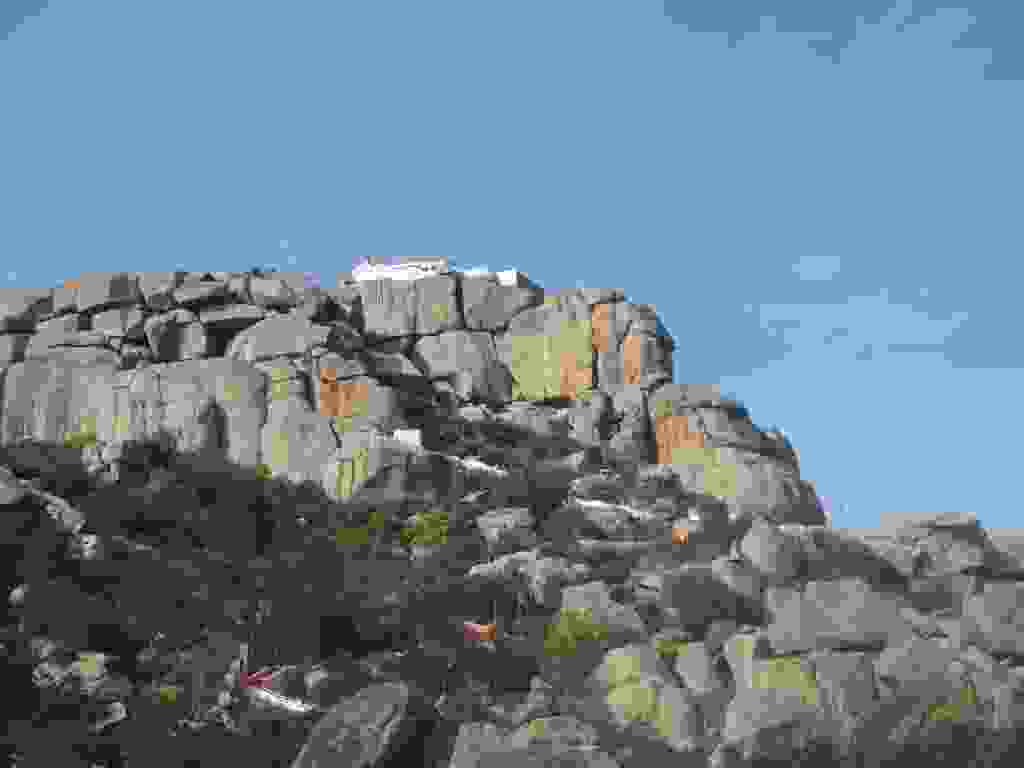
\includegraphics[width=\mywidth]{../wp-content/uploads/2015/12/PC171456-1024x768.jpg} \end{center}
\begin{center} 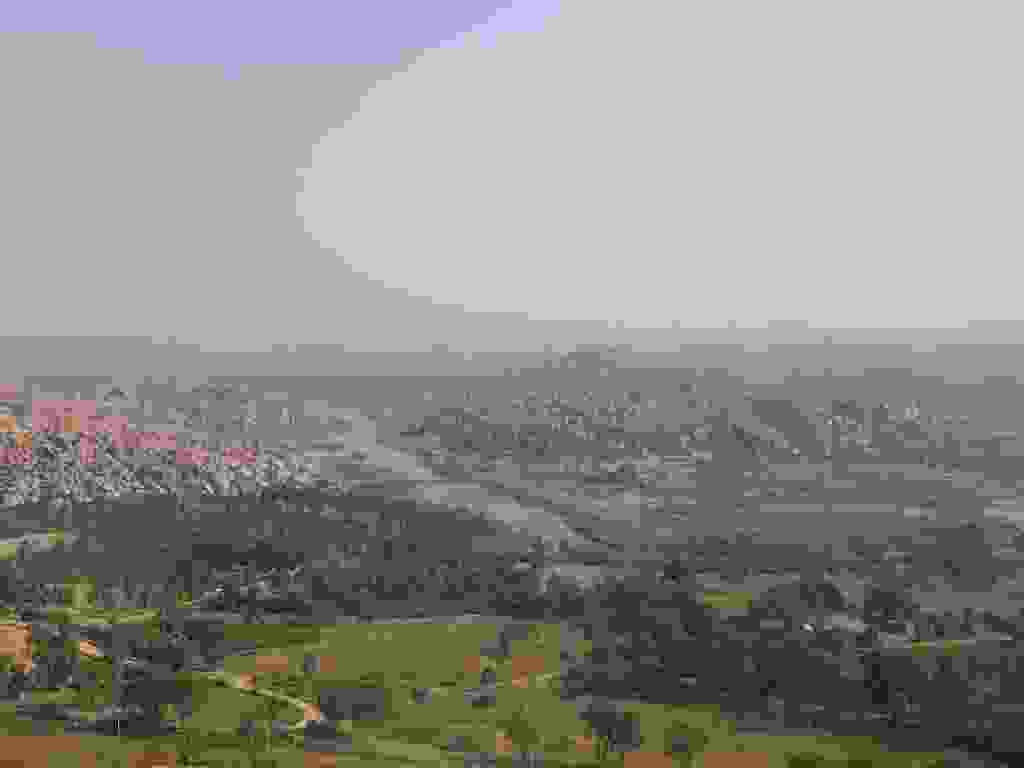
\includegraphics[width=\mywidth]{../wp-content/uploads/2015/12/PC171453-1024x768.jpg} \end{center}

Temple principal Virupaksha 
\begin{center} 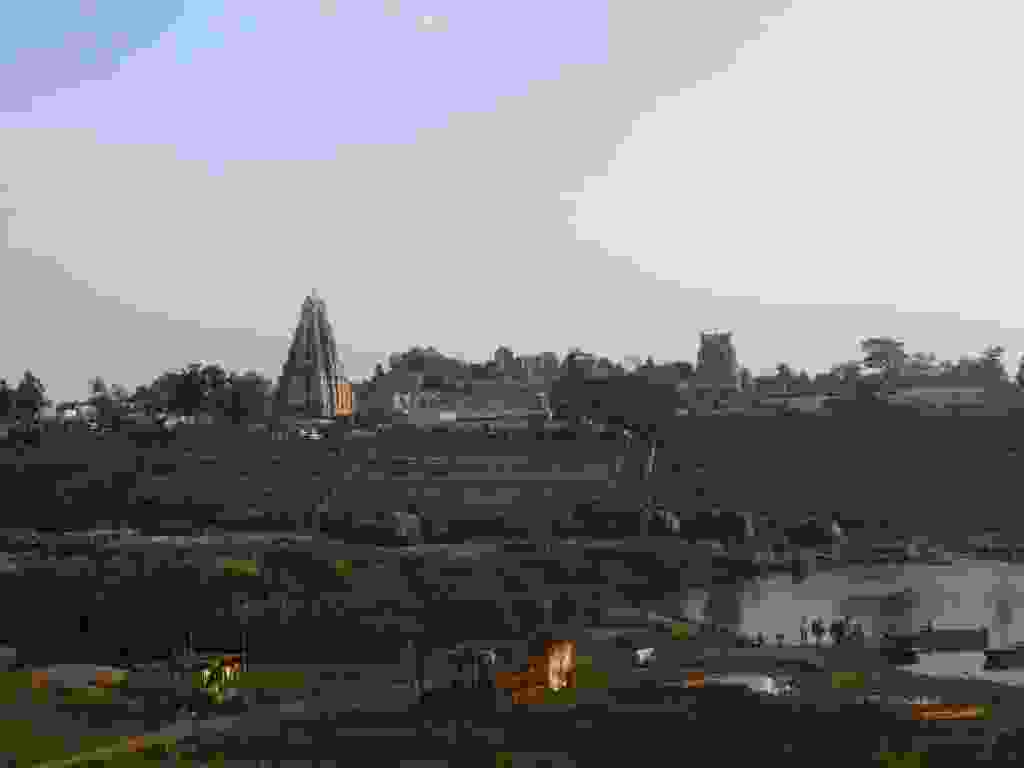
\includegraphics[width=\mywidth]{../wp-content/uploads/2015/12/PC171460-1024x768.jpg} \end{center}
\begin{center} 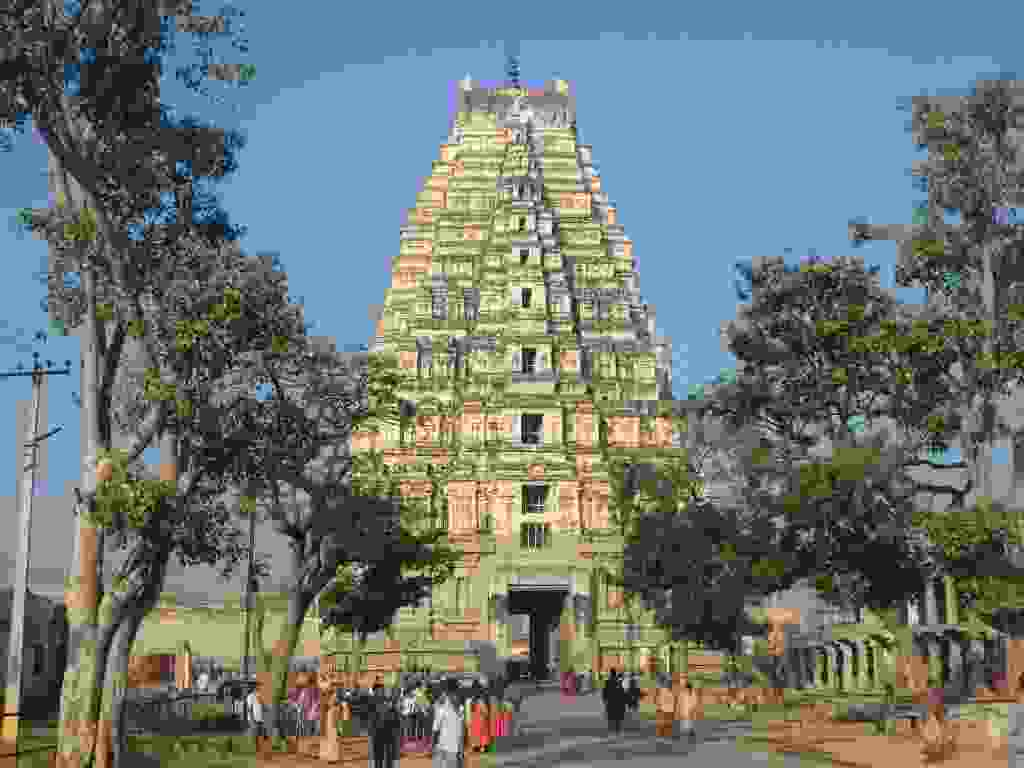
\includegraphics[width=\mywidth]{../wp-content/uploads/2015/12/PC181464-1024x768.jpg} \end{center}
\begin{center} 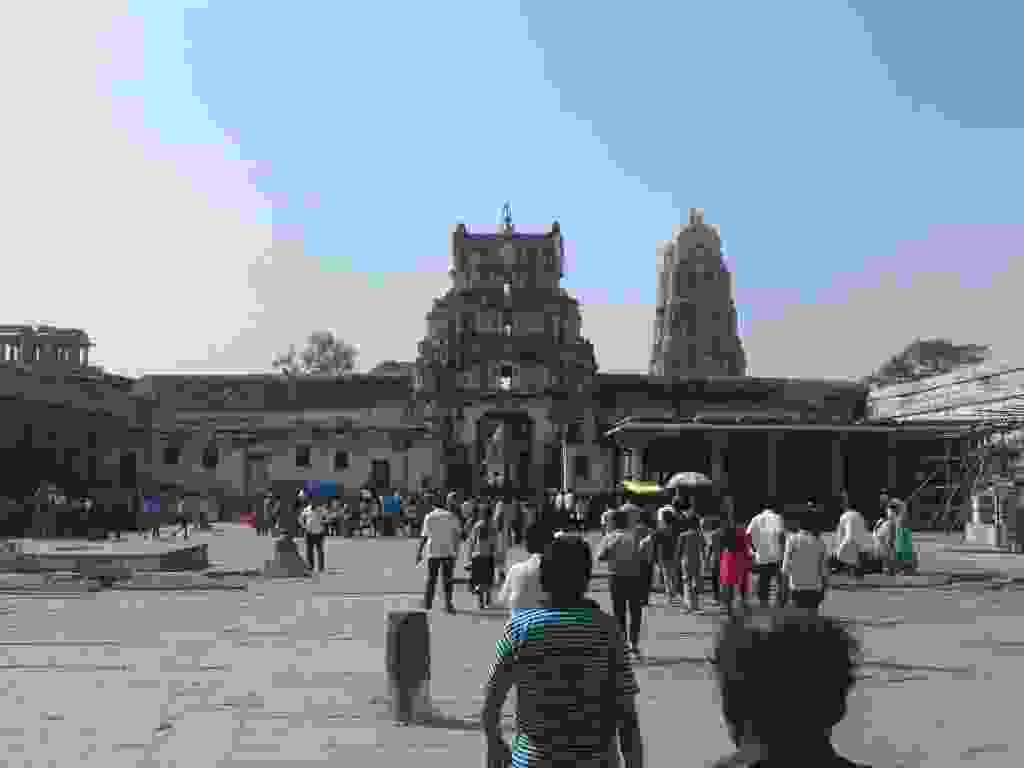
\includegraphics[width=\mywidth]{../wp-content/uploads/2015/12/PC181548-1024x768.jpg} \end{center}
\begin{center} 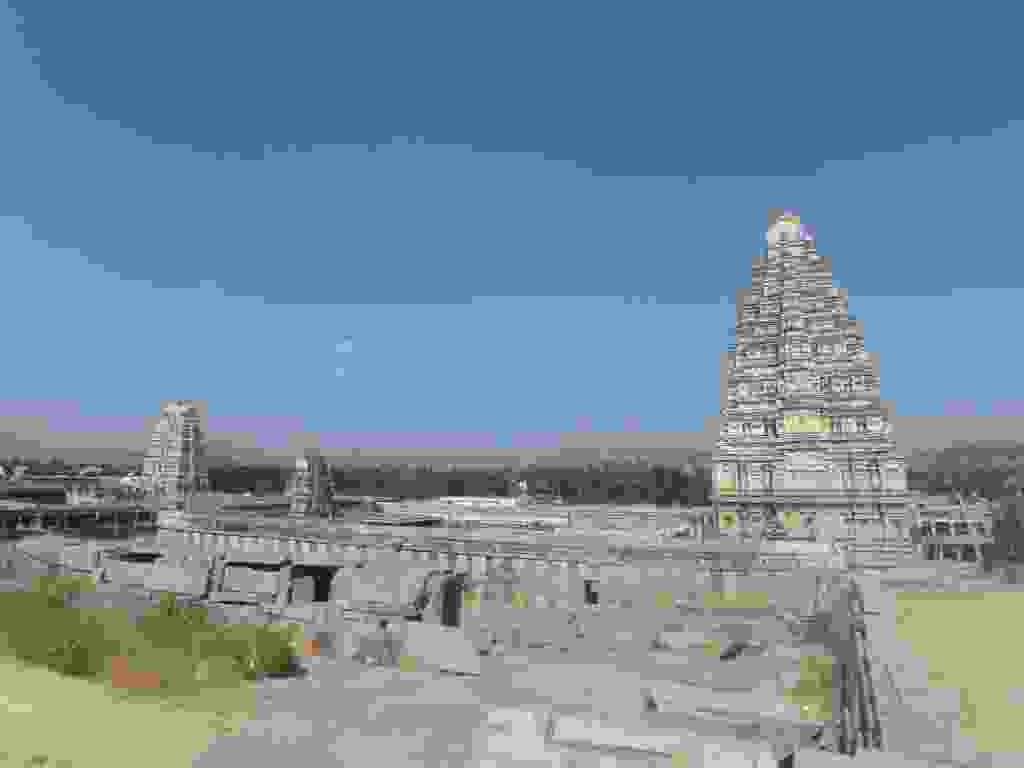
\includegraphics[width=\mywidth]{../wp-content/uploads/2015/12/PC181541-1024x768.jpg} \end{center}

Les ruines de Vijayanâgara, ancienne capitale Hindoue, éparpillées tout autour de Hampi 
\begin{center} 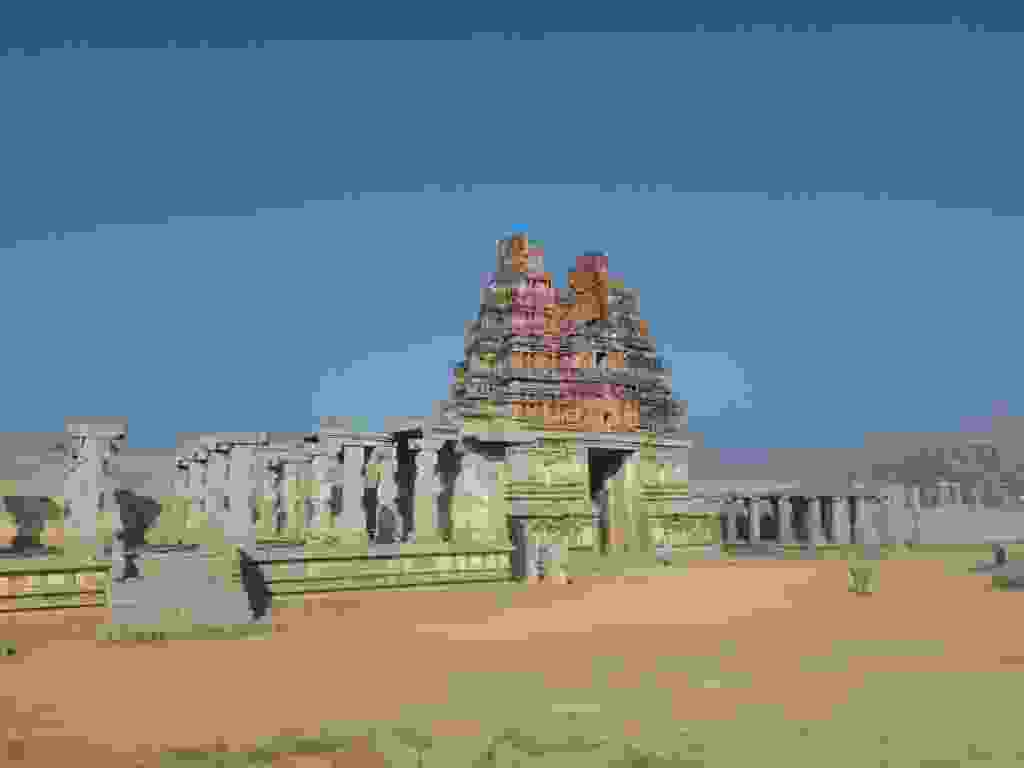
\includegraphics[width=\mywidth]{../wp-content/uploads/2015/12/PC181482-1024x768.jpg} \end{center}
\begin{center} 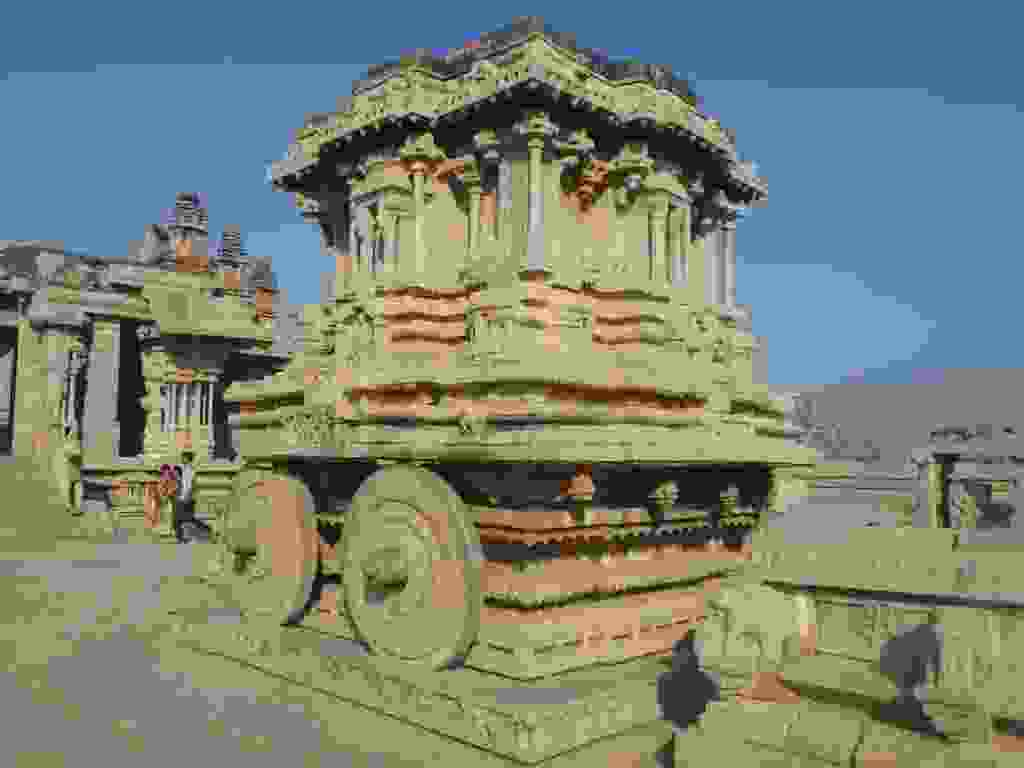
\includegraphics[width=\mywidth]{../wp-content/uploads/2015/12/PC181486-1024x768.jpg} \end{center}
\begin{center} 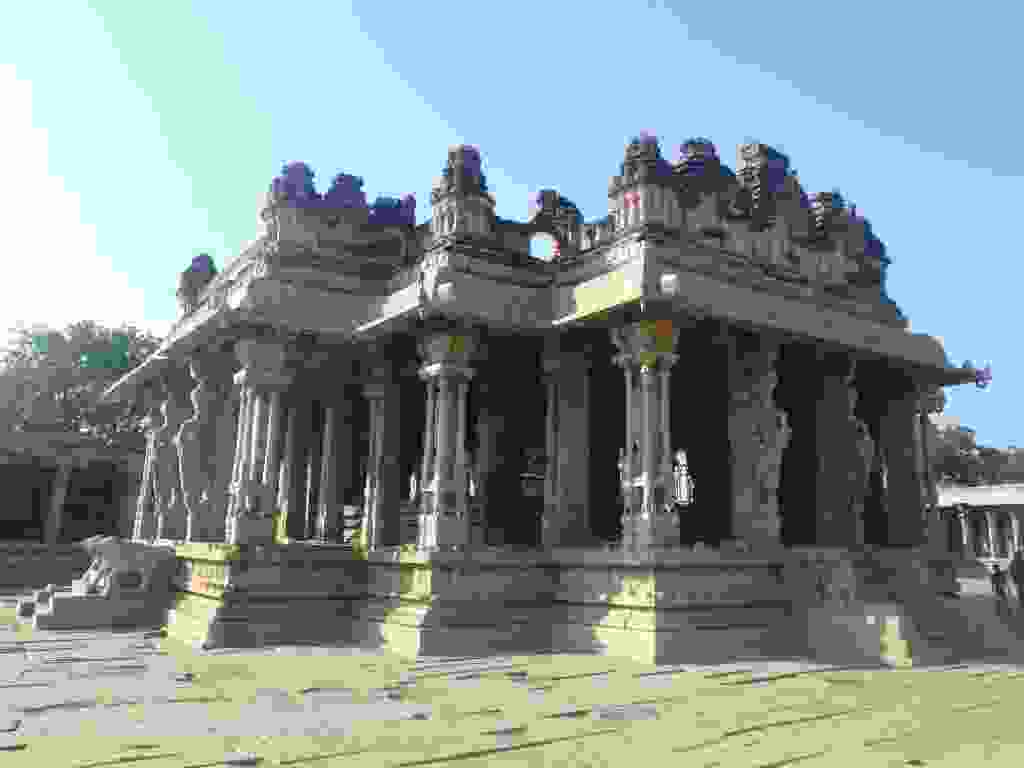
\includegraphics[width=\mywidth]{../wp-content/uploads/2015/12/PC181487-1024x768.jpg} \end{center}
\begin{center} 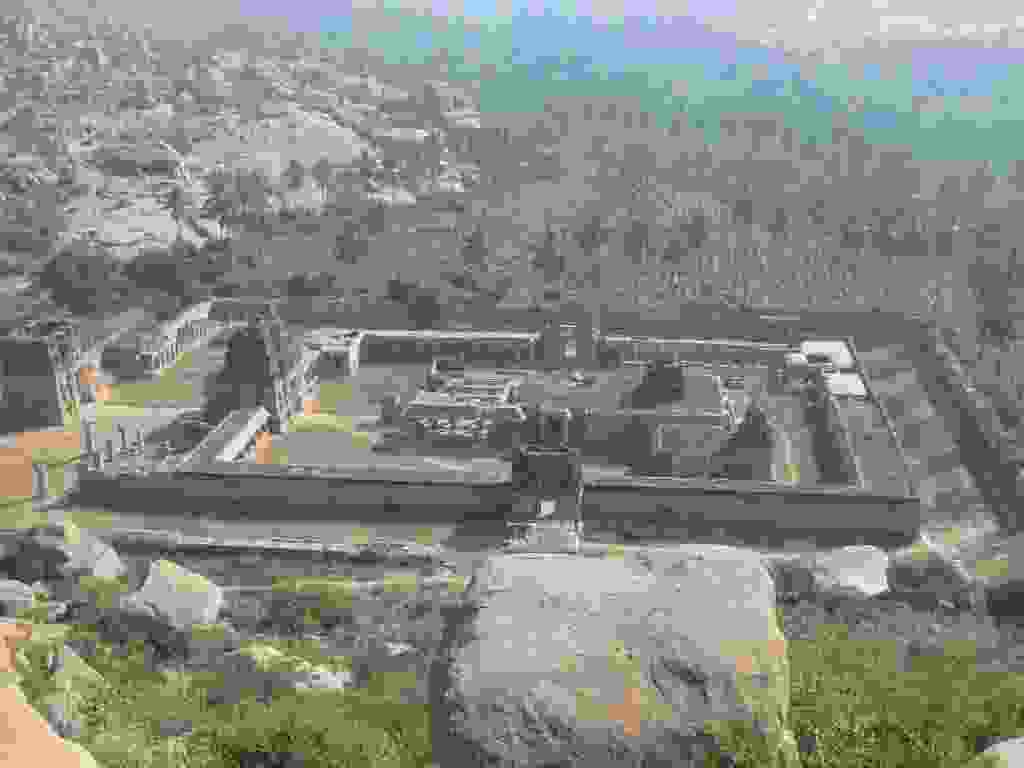
\includegraphics[width=\mywidth]{../wp-content/uploads/2015/12/PC181509-1024x768.jpg} \end{center}
\begin{center} 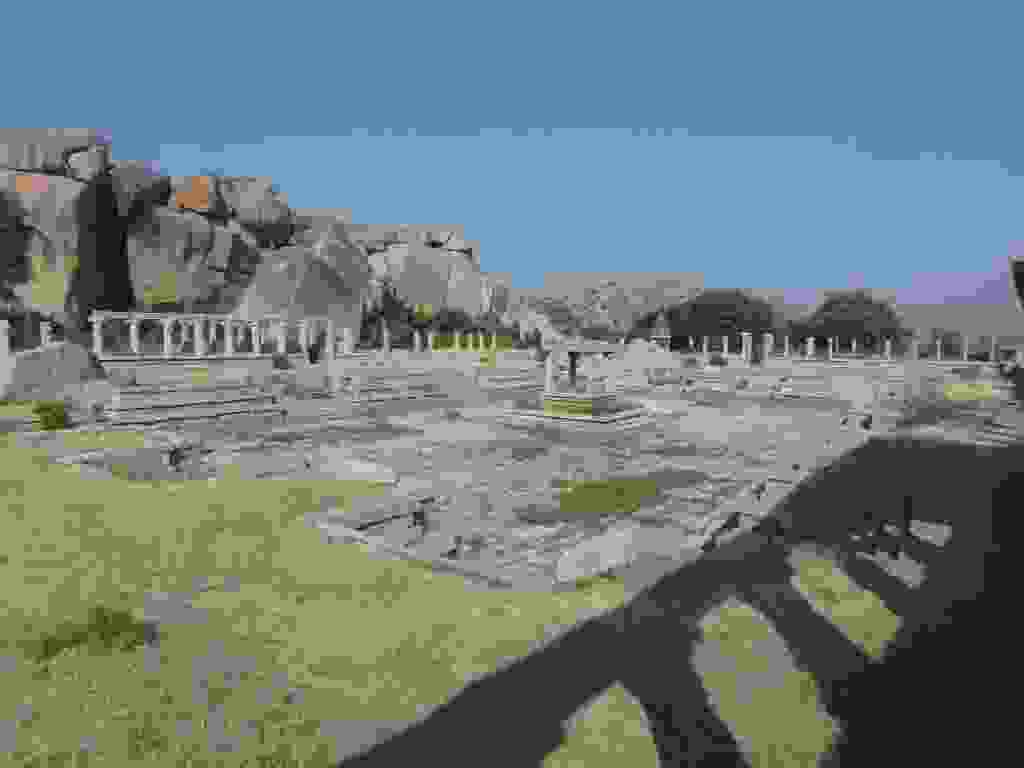
\includegraphics[width=\mywidth]{../wp-content/uploads/2015/12/PC181499-1024x768.jpg} \end{center}
\begin{center} 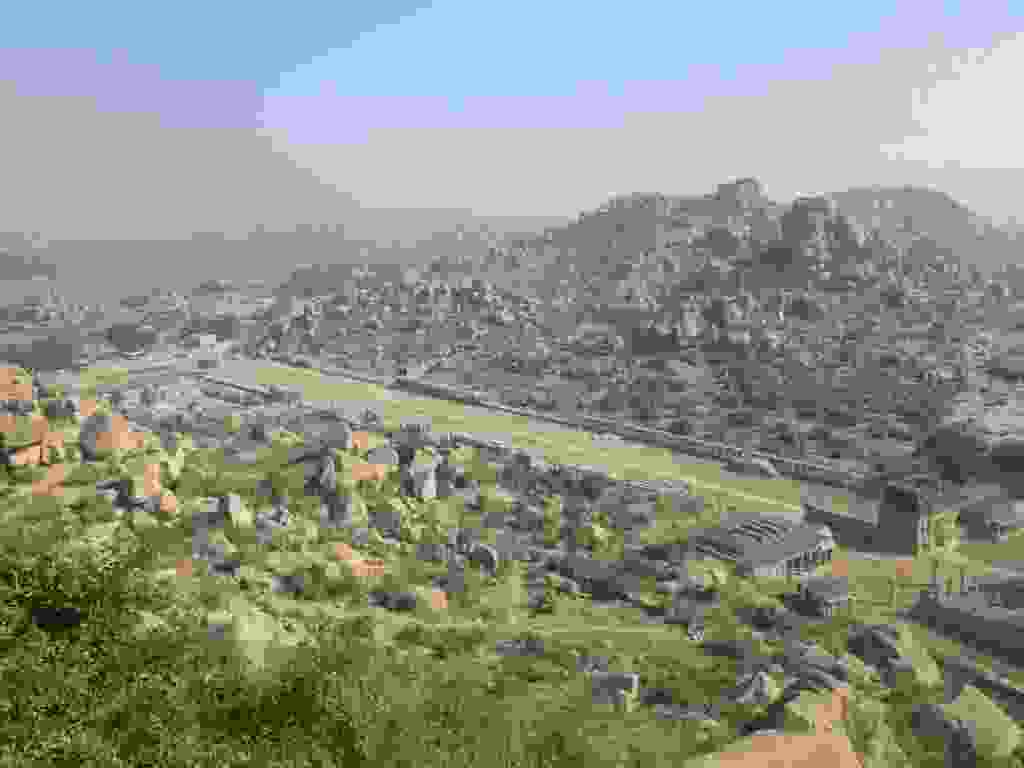
\includegraphics[width=\mywidth]{../wp-content/uploads/2015/12/PC181510-1024x768.jpg} \end{center}
\begin{center} 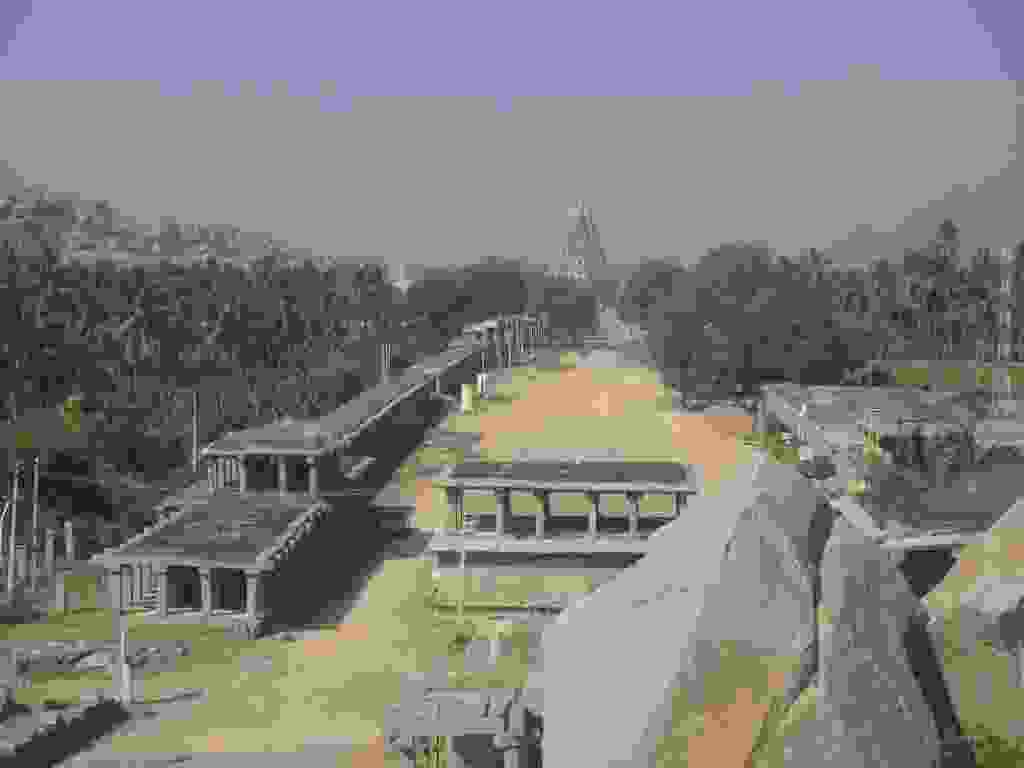
\includegraphics[width=\mywidth]{../wp-content/uploads/2015/12/PC181521-1024x768.jpg} \end{center}
\begin{center} 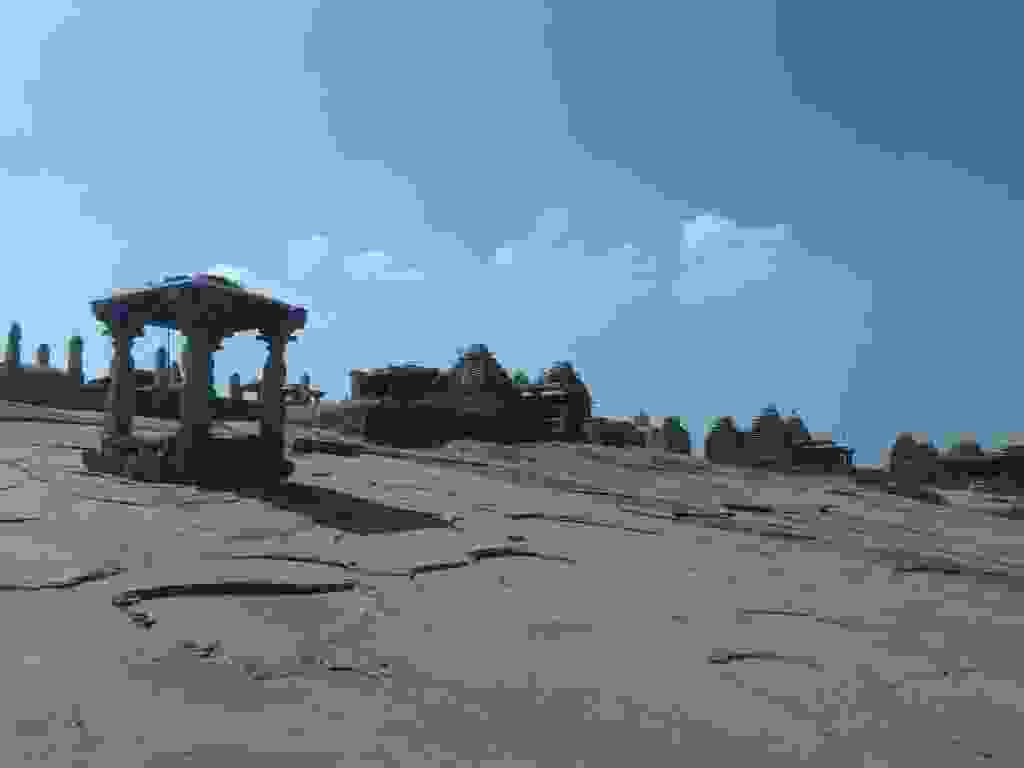
\includegraphics[width=\mywidth]{../wp-content/uploads/2015/12/PC181540-1024x768.jpg} \end{center}

Lotus Mahal
\begin{center} \includegraphics[width=\mywidth]{../wp-content/uploads/2015/12/PC181526-1024x768.jpg} \end{center}
\pagebreak

Étable pour éléphants 
\begin{center} \includegraphics[width=\mywidth]{../wp-content/uploads/2015/12/PC181529-1024x768.jpg} \end{center}

Bains de la reine 
\begin{center} \includegraphics[width=\mywidth]{../wp-content/uploads/2015/12/PC181536-1024x768.jpg} \end{center}
\pagebreak

Dernière nuit de train pour rentrer à Bangalore, je récupère le vélo laissé chez Abhijit qui m'a hébergé 
\begin{center} \includegraphics[width=\mywidth]{../wp-content/uploads/2015/12/PC191554-1024x768.jpg} \end{center}

Puis 30 km pour rejoindre l'aéroport et c'est la fin de 10 mois et demi de voyage !
